\documentclass[12pt,a4paper]{article}

\usepackage[a4paper,margin=1in]{geometry}
\usepackage{graphicx}
\usepackage{booktabs}
\usepackage{amsmath,amssymb}
\usepackage{float}
\usepackage{hyperref}
\usepackage{xurl}
\usepackage{xcolor}
\usepackage{listings}
\usepackage{enumitem}
\usepackage{fancyhdr}
\usepackage{longtable}

\hypersetup{colorlinks=true,linkcolor=blue,urlcolor=blue}

\pagestyle{fancy}
\fancyhf{}
\lhead{ICS1512}
\rhead{Machine Learning Algorithms Laboratory}
\cfoot{\thepage}

\setlength{\parskip}{0.4em}
\setlength{\parindent}{0pt}
\setlength{\headheight}{15pt}

\setlength{\floatsep}{10pt plus 2pt minus 2pt}
\setlength{\textfloatsep}{12pt plus 2pt minus 2pt}
\setlength{\intextsep}{10pt plus 2pt minus 2pt}

\setcounter{topnumber}{3}
\setcounter{bottomnumber}{3}
\setcounter{totalnumber}{4}
\renewcommand{\topfraction}{0.85}
\renewcommand{\bottomfraction}{0.85}
\renewcommand{\textfraction}{0.15}
\renewcommand{\floatpagefraction}{0.8}

\lstset{
language=Python,
basicstyle=\ttfamily\small,
numbers=left,
frame=single,
breaklines=true,
showstringspaces=false
}

\begin{document}

\begin{tabular}{|p{4cm}|p{11cm}|}
\hline
Experiment No. & 1 \\ \hline
Experiment Title & Working with Python Packages: NumPy, SciPy, Scikit-Learn, Matplotlib, and Pandas (Loan Prediction Dataset) \\ \hline
Student Name & Srinivasan M \\ \hline
Register Number & 3122247001063 \\ \hline
Faculty & Dr. Poreddy Ajay Kumar Reddy \\ \hline
Submission Date & \today \\ \hline
\end{tabular}

\vspace{0.3cm}

\section{Objective}
The core goals of this laboratory exercise comprise:
\begin{itemize}[noitemsep]
    \item Master fundamental data manipulation, array operations, statistical routines, and data visualization primitives across the standard Python scientific stack (NumPy, SciPy, Scikit-Learn, Matplotlib, Pandas).
    \item Construct a reusable, automated Exploratory Data Analysis (EDA) engine capable of ingesting arbitrary tabular data and extracting statistical parameters, missing value profiles, and distribution visual shapes.
    \item Categorize five standard benchmark datasets (Iris, Loan Amount Prediction, Diabetes, Email Spam, MNIST) by ML paradigm, target variable characteristics, feature selection methodologies, and model choices.
    \item Perform full automated EDA on the continuous \textbf{Loan Amount Prediction Dataset}, analyzing generated visual outputs and statistical summaries.
\end{itemize}

\section{Problem Statement}
Prior to modeling real-world tabular data, data practitioners must perform comprehensive data auditing to identify skewness, unexpected multi-modal distributions, correlation structures, and missing entries. Manual analysis for every newly ingested dataset introduces code redundancy and inefficiency. This experiment addresses the challenge by implementing an end-to-end automated EDA tool using Python's numerical stack to load datasets, generate statistical summaries, and save informative visual representations. Furthermore, standard benchmark datasets are mapped into supervised and unsupervised paradigms to structure future model selection.

\section{Dataset Description}
The empirical analysis in this section focuses on the **Loan Amount Prediction Dataset**.

\begin{longtable}{|p{6cm}|p{8cm}|}
\hline
Dataset Name & Loan Amount Prediction Dataset \\ \hline
Dataset Source & UCI Machine Learning Repository / Kaggle \\ \hline
Number of Samples & 614 \\ \hline
Number of Features & 13 (5 continuous/discrete numerical, 8 categorical) \\ \hline
Number of Classes & N/A (Continuous Target: LoanAmount) \\ \hline
Missing Values & Present (Gender, Married, Dependents, Self\_Employed, LoanAmount, Loan\_Amount\_Term, Credit\_History) \\ \hline
Train-Test Split & N/A (Exploratory Analysis Phase) \\ \hline
\end{longtable}

The dataset consists of the following attributes:
\begin{itemize}[noitemsep]
    \item \texttt{Loan\_ID}: Unique identifier string for each loan application.
    \item \texttt{Gender}: Applicant gender (Male / Female).
    \item \texttt{Married}: Marital status of the applicant (Yes / No).
    \item \texttt{Dependents}: Count of financial dependents (0, 1, 2, 3+).
    \item \texttt{Education}: Educational level (Graduate / Not Graduate).
    \item \texttt{Self\_Employed}: Employment type indicator (Yes / No).
    \item \texttt{ApplicantIncome}: Primary applicant monthly income in USD.
    \item \texttt{CoapplicantIncome}: Additional co-applicant monthly income in USD.
    \item \texttt{LoanAmount}: Requested credit amount in thousands of USD (Target).
    \item \texttt{Loan\_Amount\_Term}: Loan repayment period expressed in months.
    \item \texttt{Credit\_History}: Credit guideline compliance indicator (1.0 = positive, 0.0 = negative).
    \item \texttt{Property\_Area}: Geographical location of property (Urban / Semiurban / Rural).
    \item \texttt{Loan\_Status}: Historical loan approval status (Y / N).
\end{itemize}

\section{Exploratory Data Analysis}
The automated EDA framework generated 28 diagnostic graphics saved in the \texttt{figures\_loan/} directory. Individual figures and corresponding analytical inferences are presented below.

\subsection{Histograms of Numerical Features}

\begin{figure}[H]
\centering
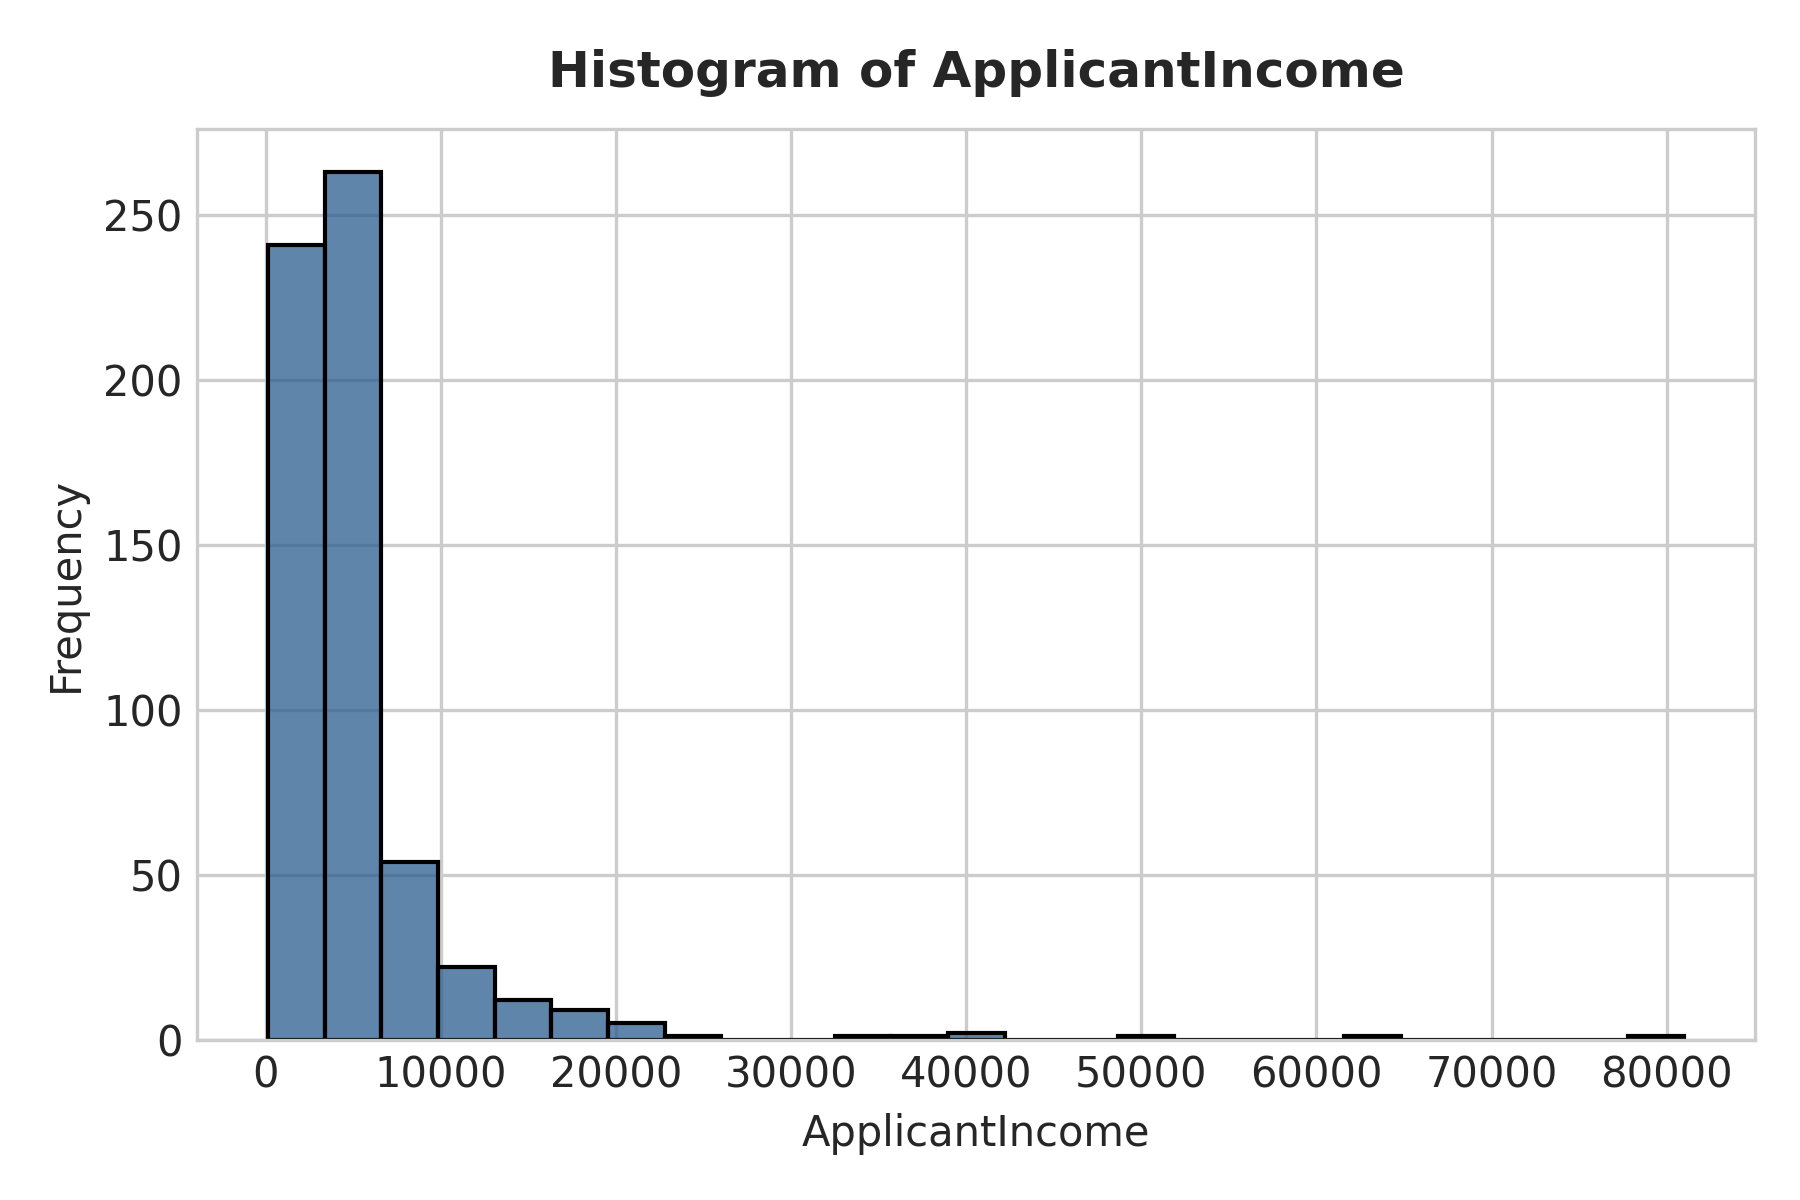
\includegraphics[width=0.75\linewidth]{figures_loan/hist_ApplicantIncome.png}
\caption{Histogram of Applicant Income}
\label{fig:hist_app_income}
\end{figure}
\textbf{Inference:} The applicant income distribution exhibits pronounced right skewness. Most applicants report monthly incomes below \$10,000, while a thin tail reaches toward \$80,000. Applying a logarithmic transformation prior to model fitting is advisable to mitigate variance instability.

\begin{figure}[H]
\centering
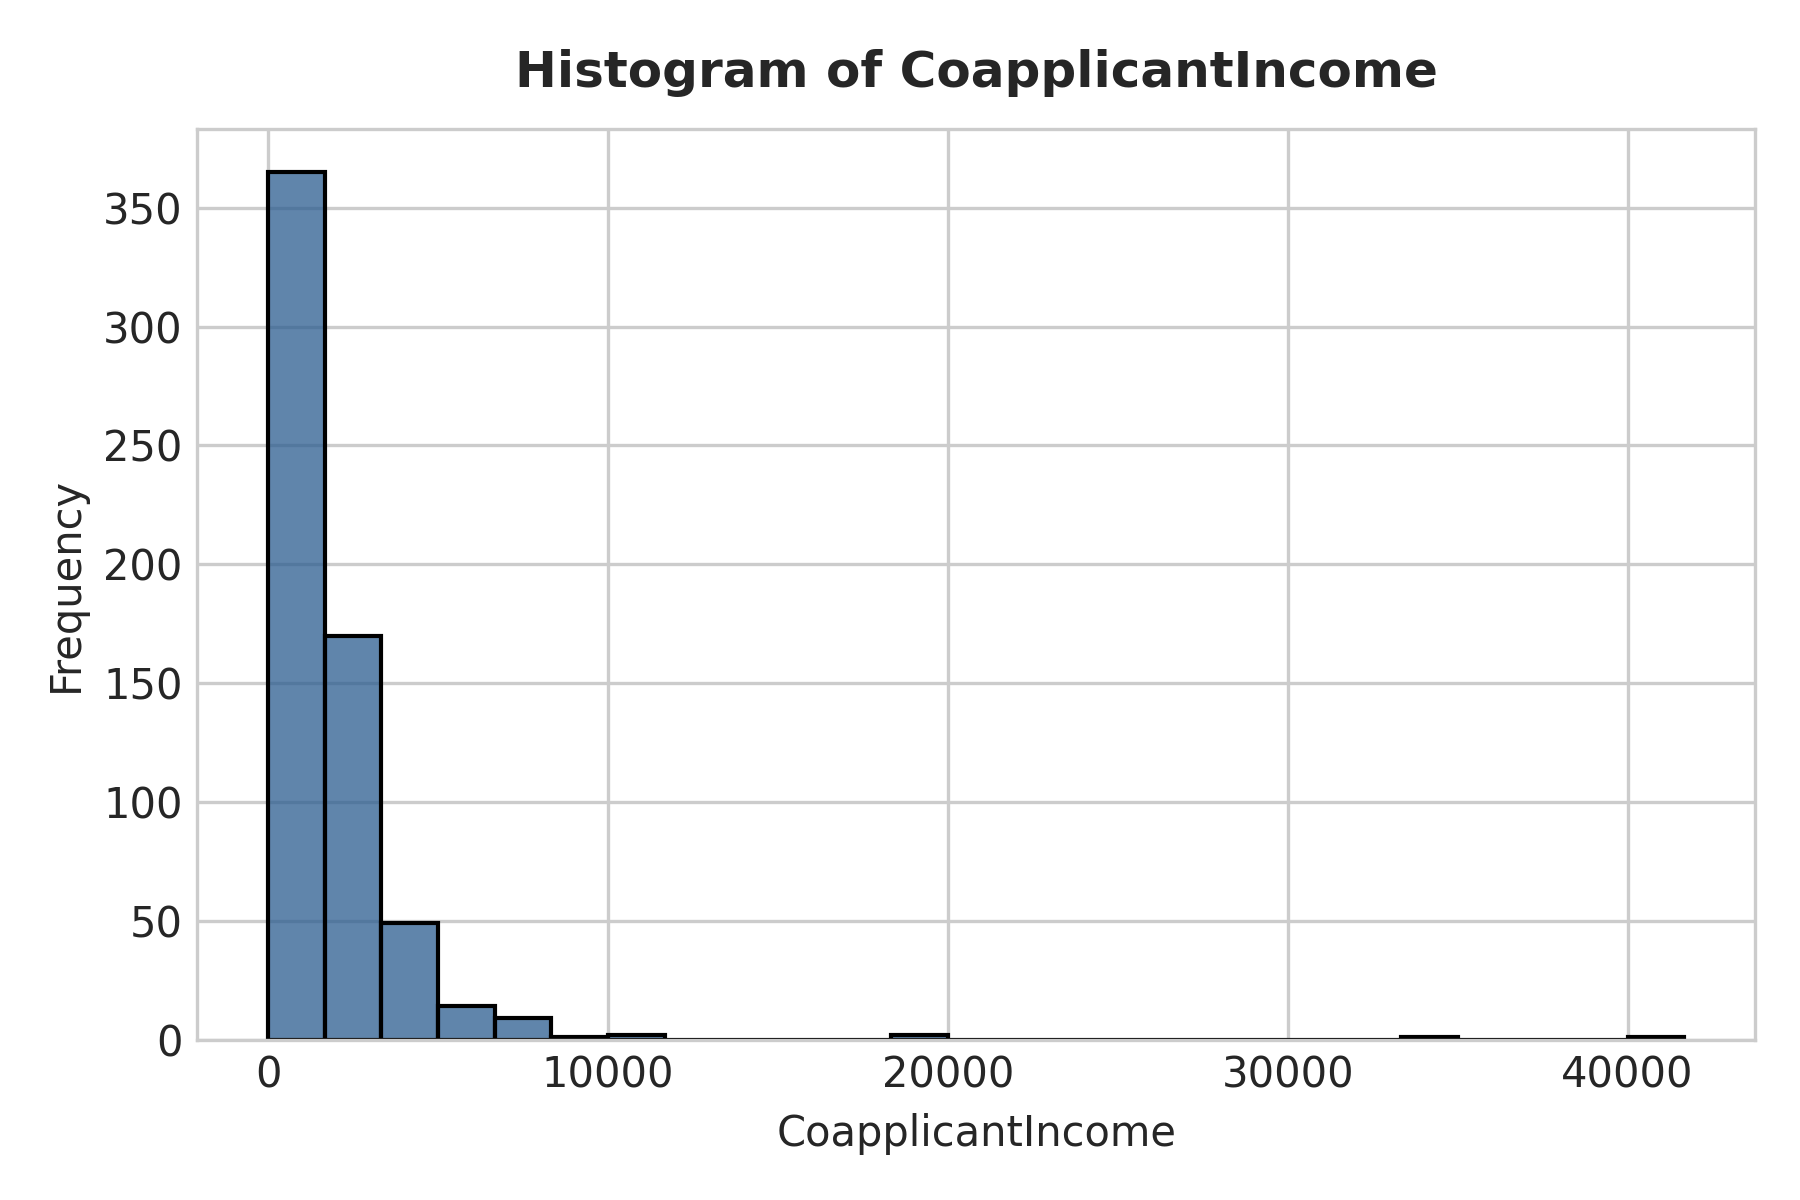
\includegraphics[width=0.75\linewidth]{figures_loan/hist_CoapplicantIncome.png}
\caption{Histogram of Co-applicant Income}
\label{fig:hist_coapp_income}
\end{figure}
\textbf{Inference:} Co-applicant income features a massive spike at \$0, representing applications submitted without a co-borrower. Non-zero entries show positive skewness stretching up to \$40,000.

\begin{figure}[H]
\centering
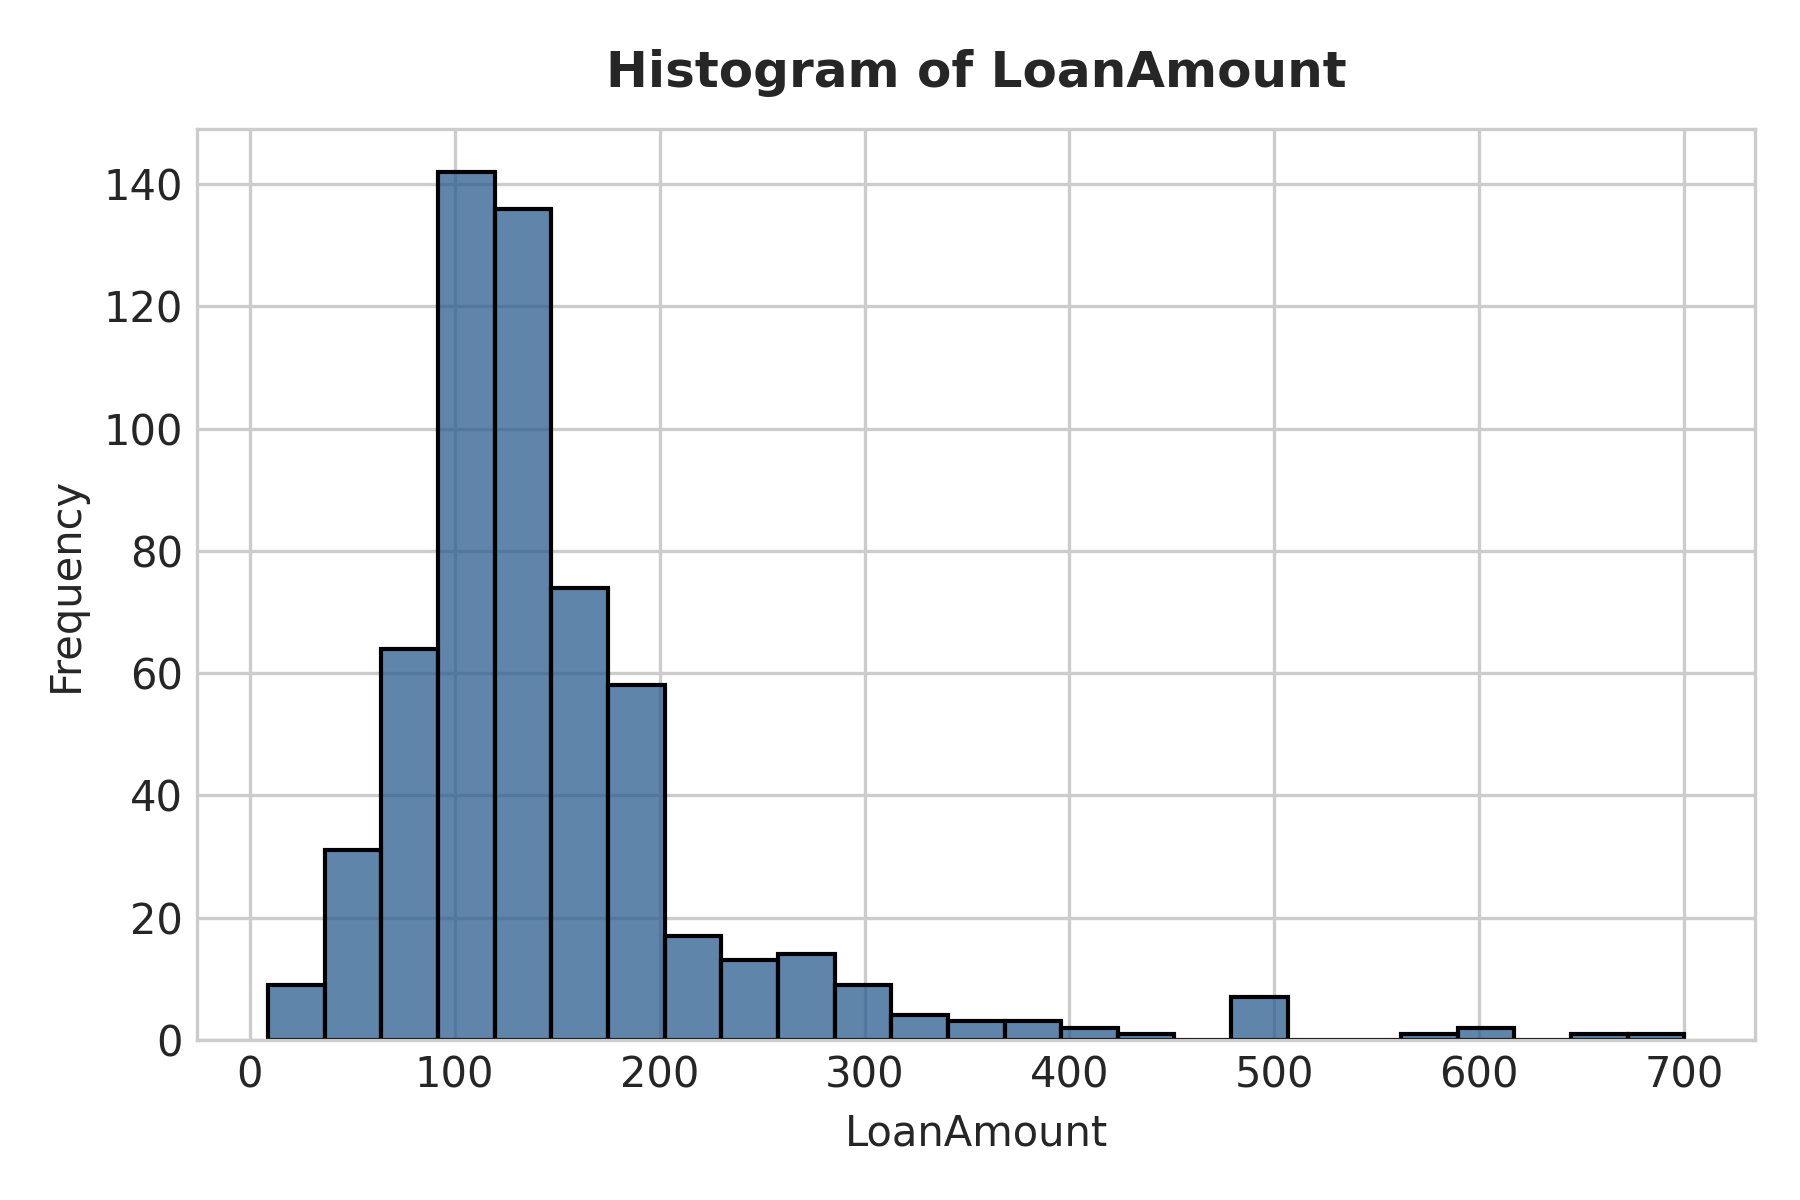
\includegraphics[width=0.75\linewidth]{figures_loan/hist_LoanAmount.png}
\caption{Histogram of Loan Amount}
\label{fig:hist_loan_amount}
\end{figure}
\textbf{Inference:} The target variable (\texttt{LoanAmount}) displays a unimodal distribution centered around \$130,000-\$150,000, with minor right-skewness and values spanning \$9,000 to \$700,000.

\begin{figure}[H]
\centering
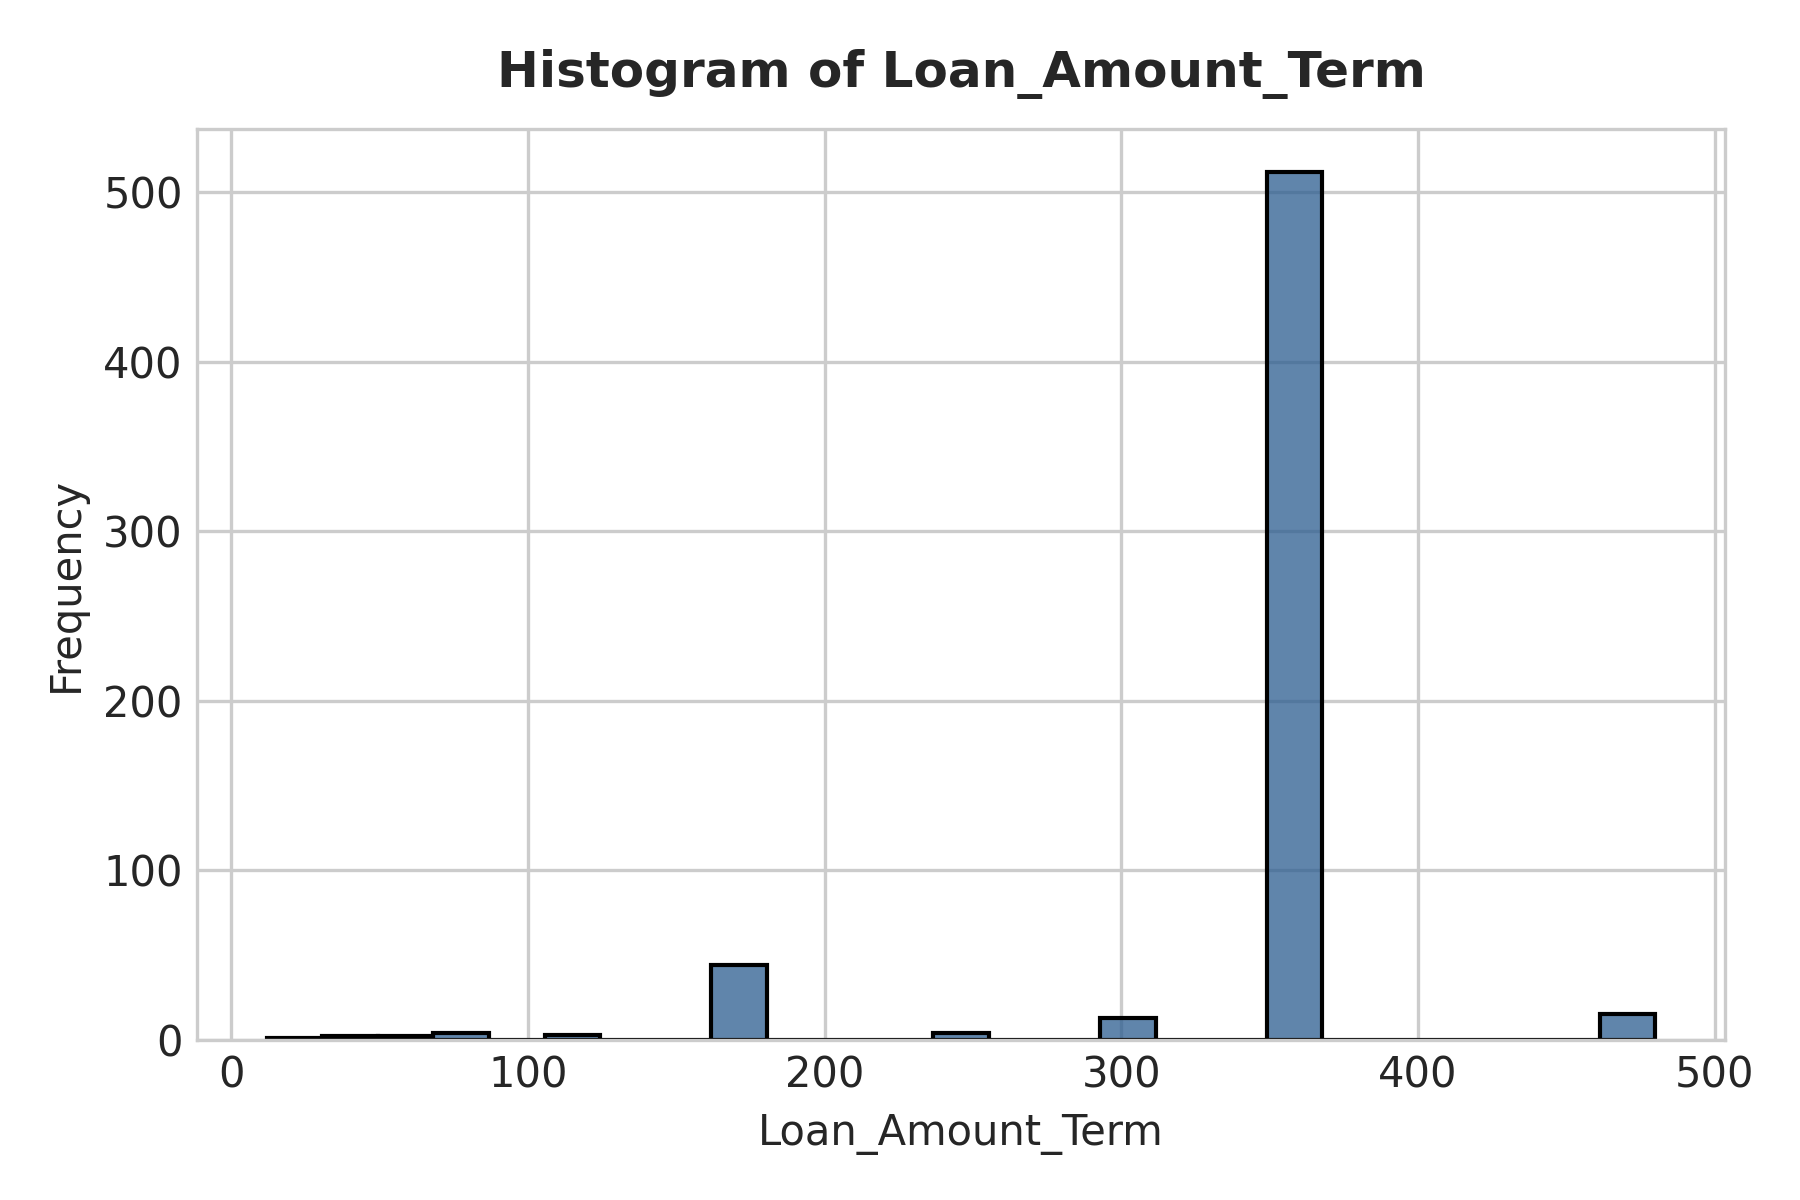
\includegraphics[width=0.75\linewidth]{figures_loan/hist_Loan_Amount_Term.png}
\caption{Histogram of Loan Amount Term}
\label{fig:hist_loan_term}
\end{figure}
\textbf{Inference:} The repayment term distribution is discrete, dominated heavily by the standard 360-month (30-year) mortgage period. Intermediate terms like 180 or 240 months appear far less frequently.

\begin{figure}[H]
\centering
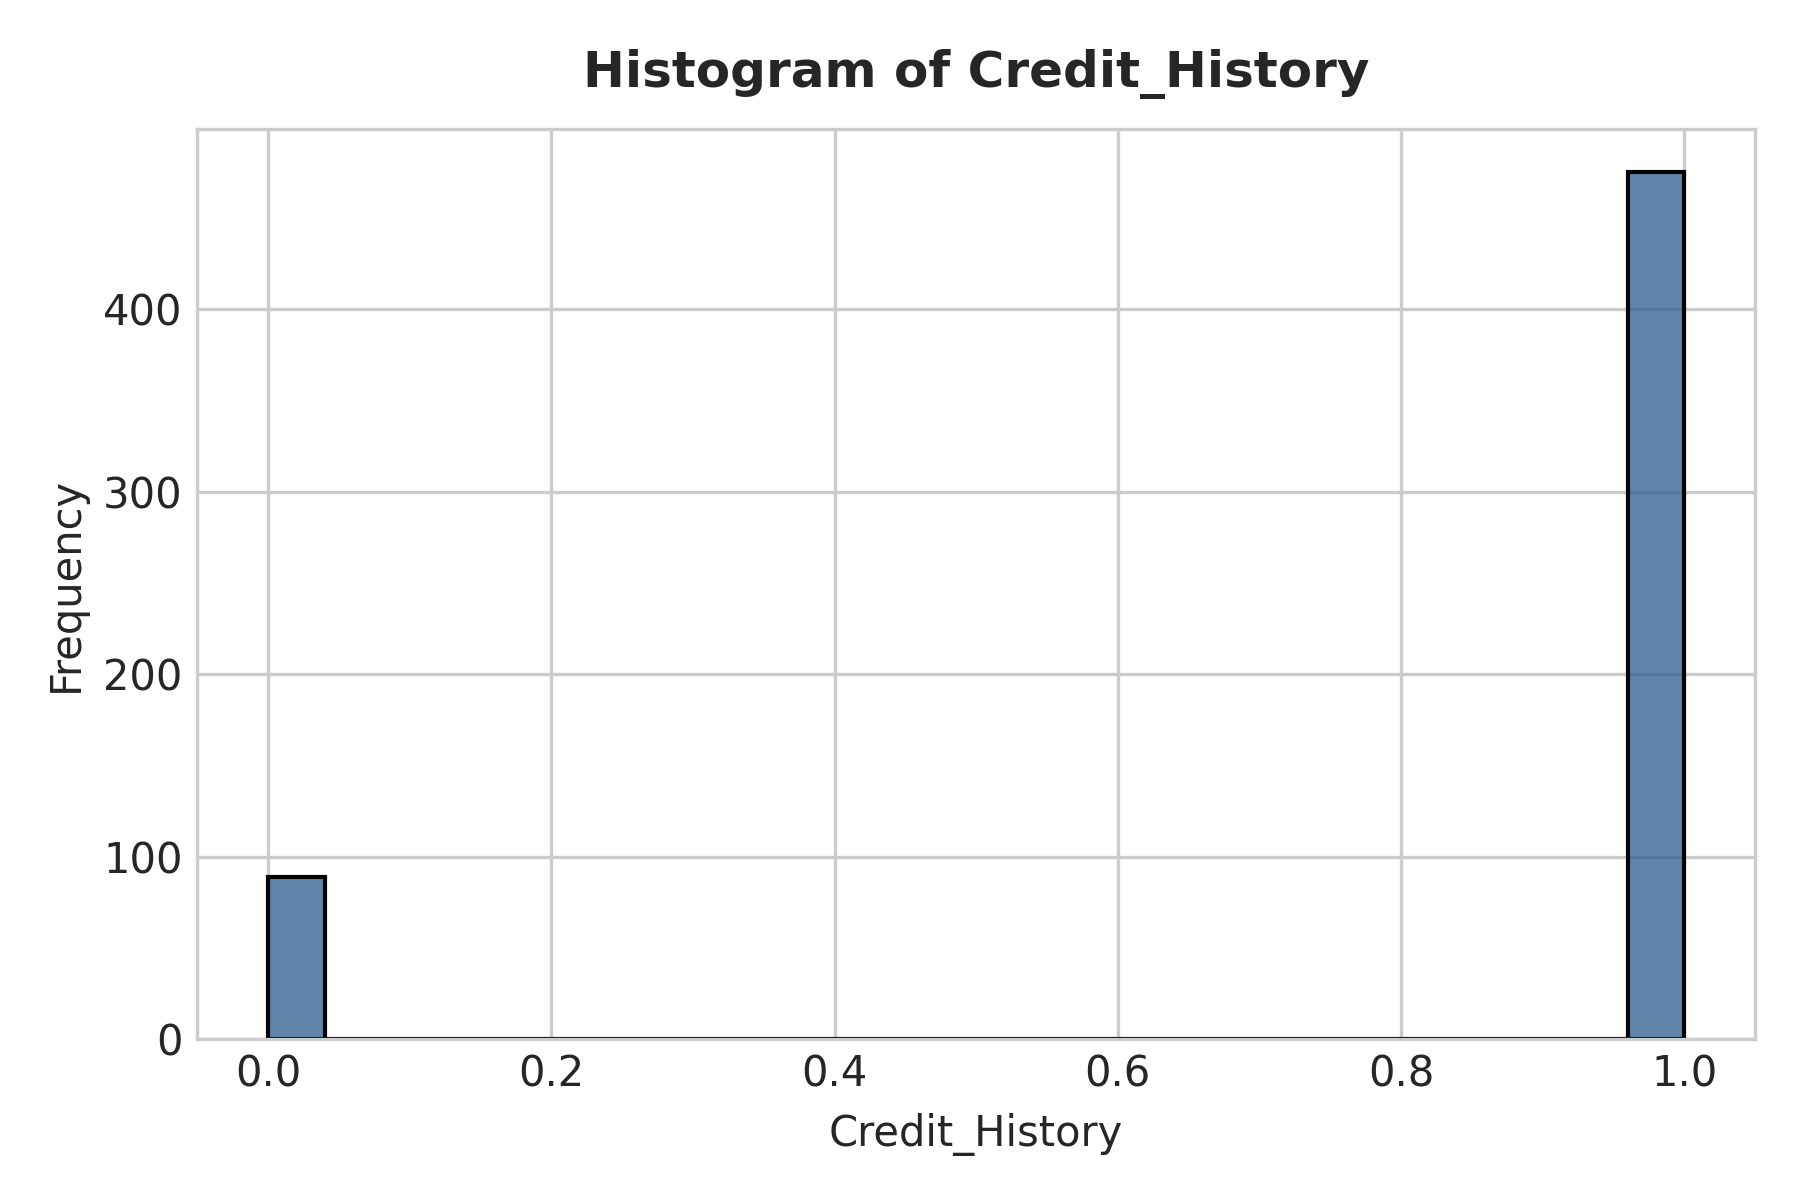
\includegraphics[width=0.75\linewidth]{figures_loan/hist_Credit_History.png}
\caption{Histogram of Credit History}
\label{fig:hist_credit_history}
\end{figure}
\textbf{Inference:} Credit history records fall into two binary bins. A significant majority of applicants possess a positive history (\texttt{Credit\_History} = 1.0), indicating potential class imbalance in this attribute.

\subsection{Box Plots of Numerical Features}

\begin{figure}[H]
\centering
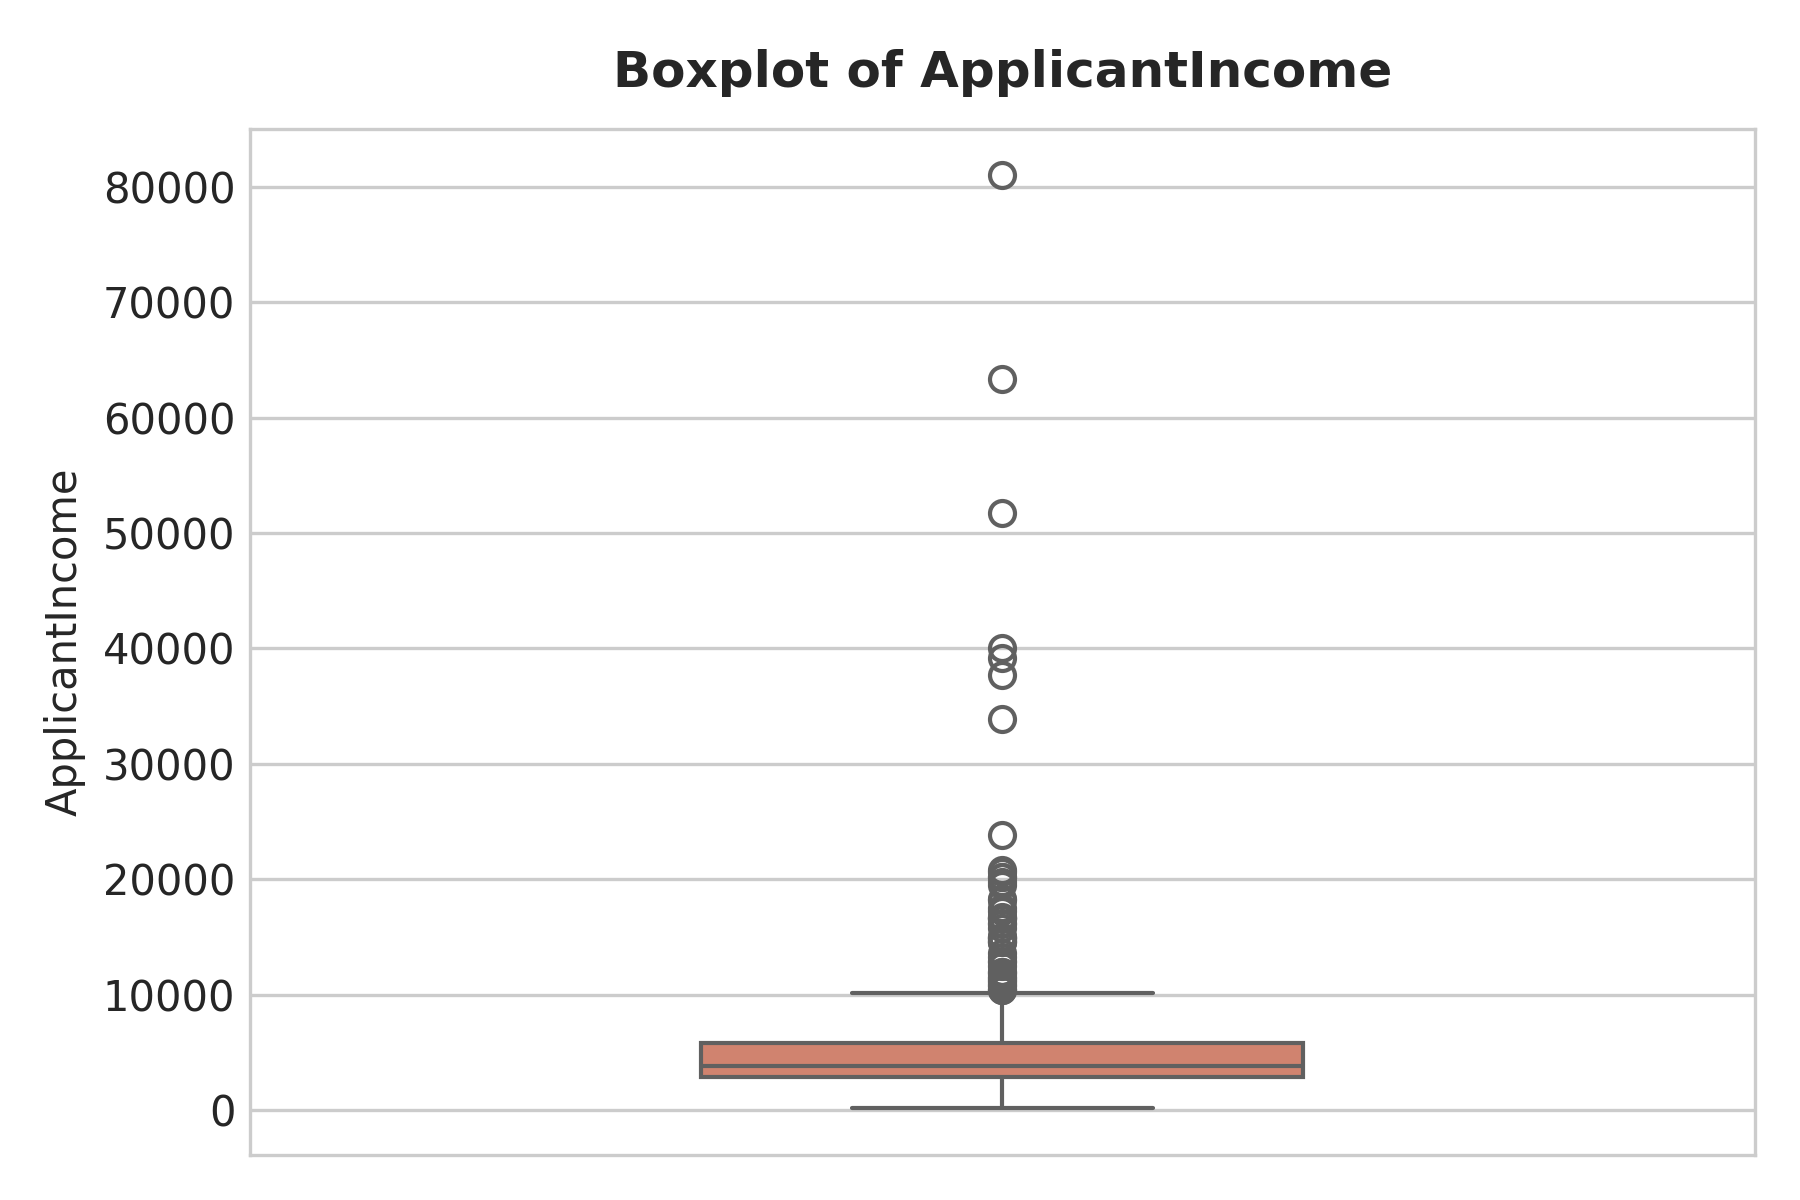
\includegraphics[width=0.75\linewidth]{figures_loan/box_ApplicantIncome.png}
\caption{Box Plot of Applicant Income}
\label{fig:box_app_income}
\end{figure}
\textbf{Inference:} The boxplot displays a compact interquartile range (IQR) with median income around \$3,812. Numerous upper outliers extend beyond the whisker bound, confirming high income dispersion.

\begin{figure}[H]
\centering
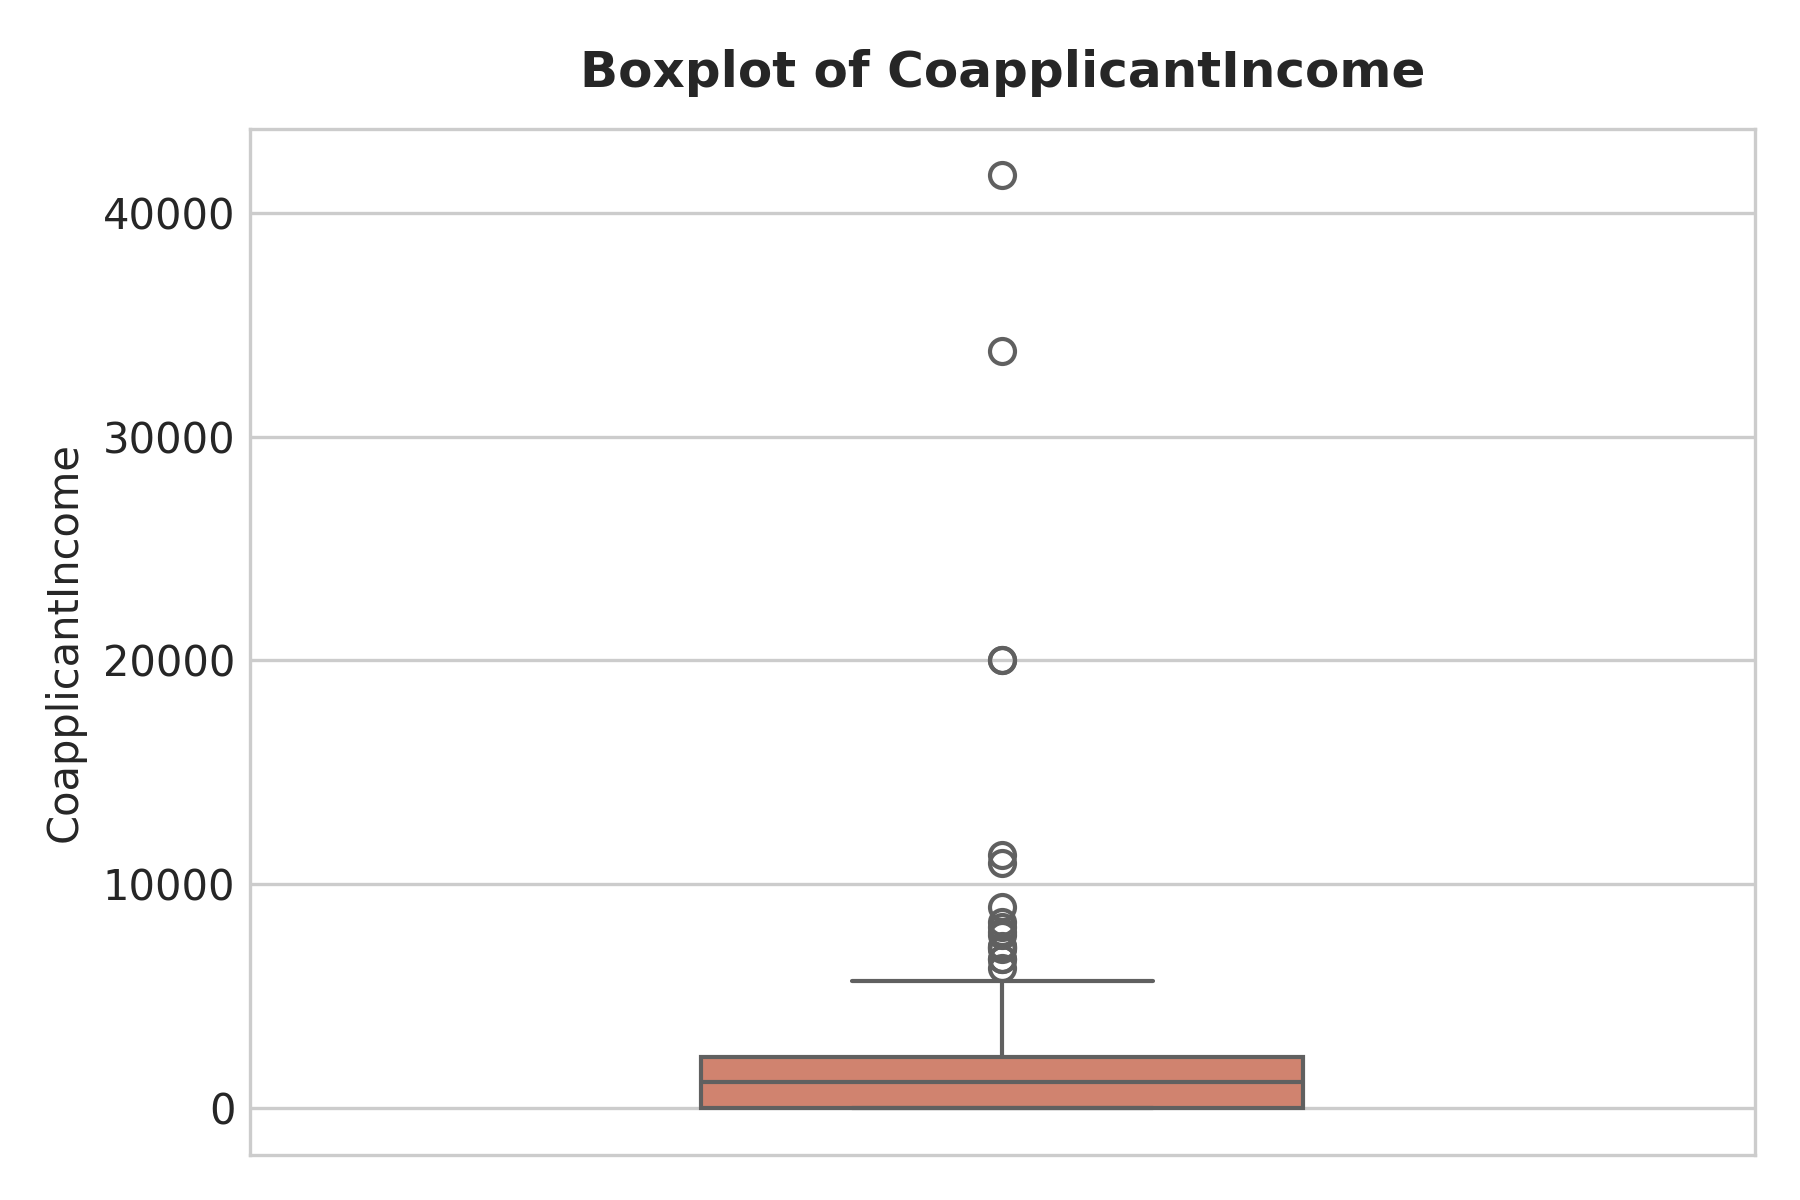
\includegraphics[width=0.75\linewidth]{figures_loan/box_CoapplicantIncome.png}
\caption{Box Plot of Co-applicant Income}
\label{fig:box_coapp_income}
\end{figure}
\textbf{Inference:} Co-applicant income shows a low median near \$1,188, alongside multiple extreme values exceeding \$10,000.

\begin{figure}[H]
\centering
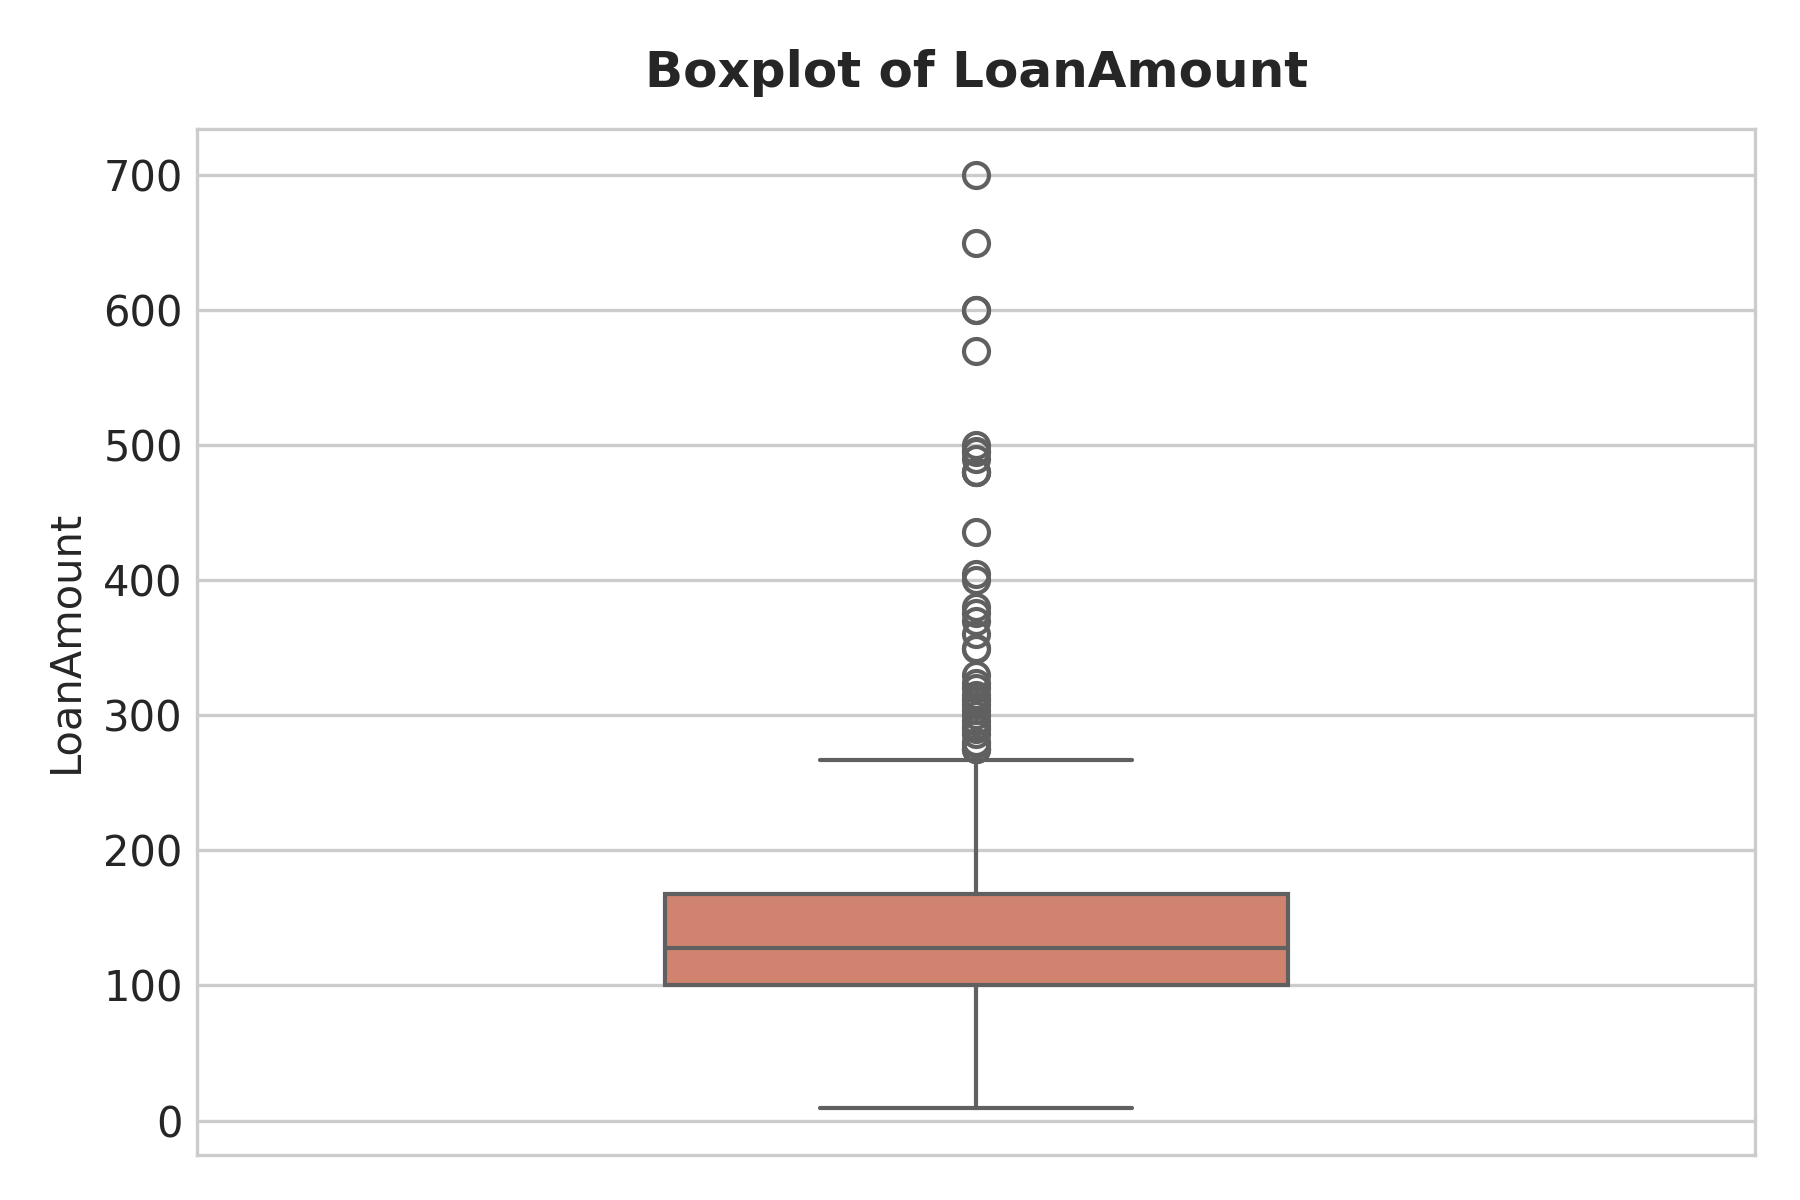
\includegraphics[width=0.75\linewidth]{figures_loan/box_LoanAmount.png}
\caption{Box Plot of Loan Amount}
\label{fig:box_loan_amount}
\end{figure}
\textbf{Inference:} The loan amount median sits near \$128,000. Outliers above \$260,000 highlight large loan applications requiring robust scaling during preprocessing.

\begin{figure}[H]
\centering
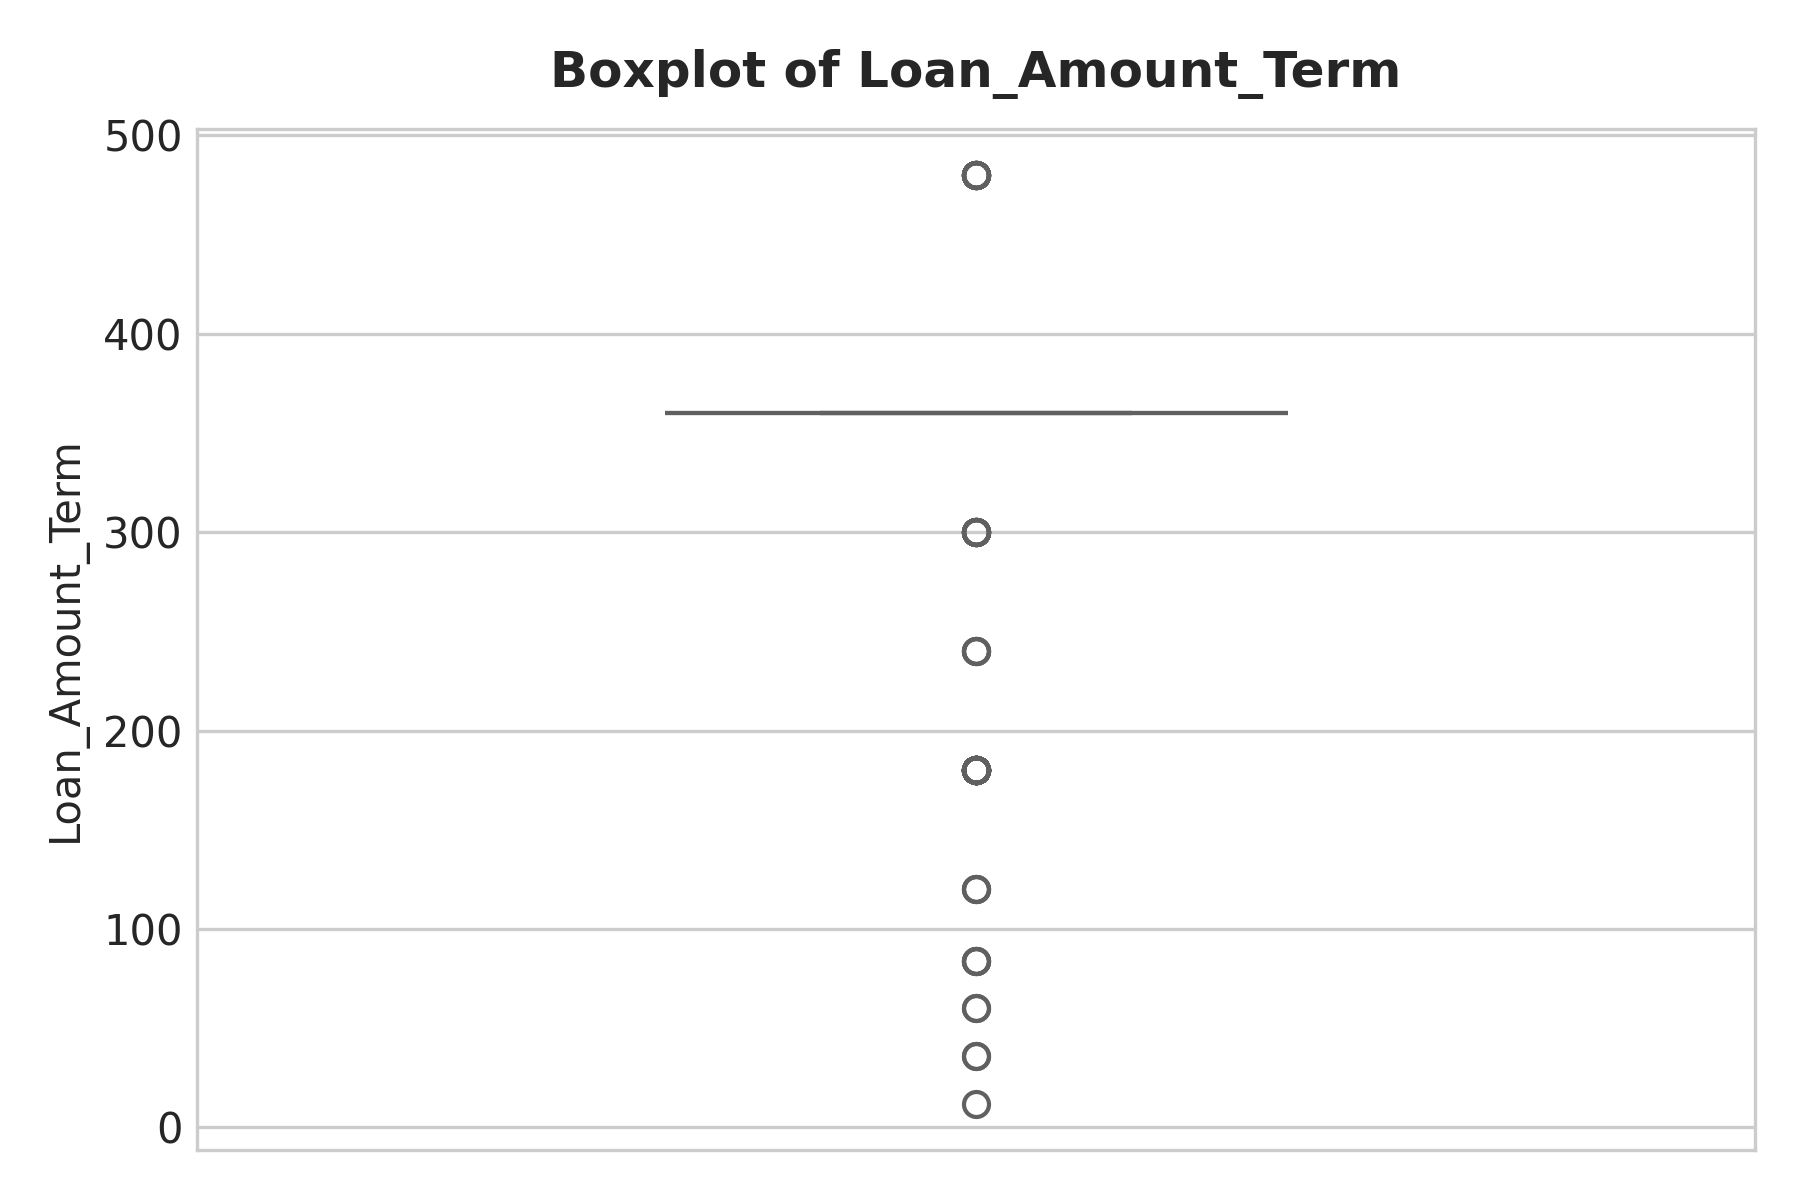
\includegraphics[width=0.75\linewidth]{figures_loan/box_Loan_Amount_Term.png}
\caption{Box Plot of Loan Amount Term}
\label{fig:box_loan_term}
\end{figure}
\textbf{Inference:} The term variable is concentrated at 360 months. Non-standard loan durations (12 to 240 months and 480 months) appear as statistical outliers in the plot.

\begin{figure}[H]
\centering
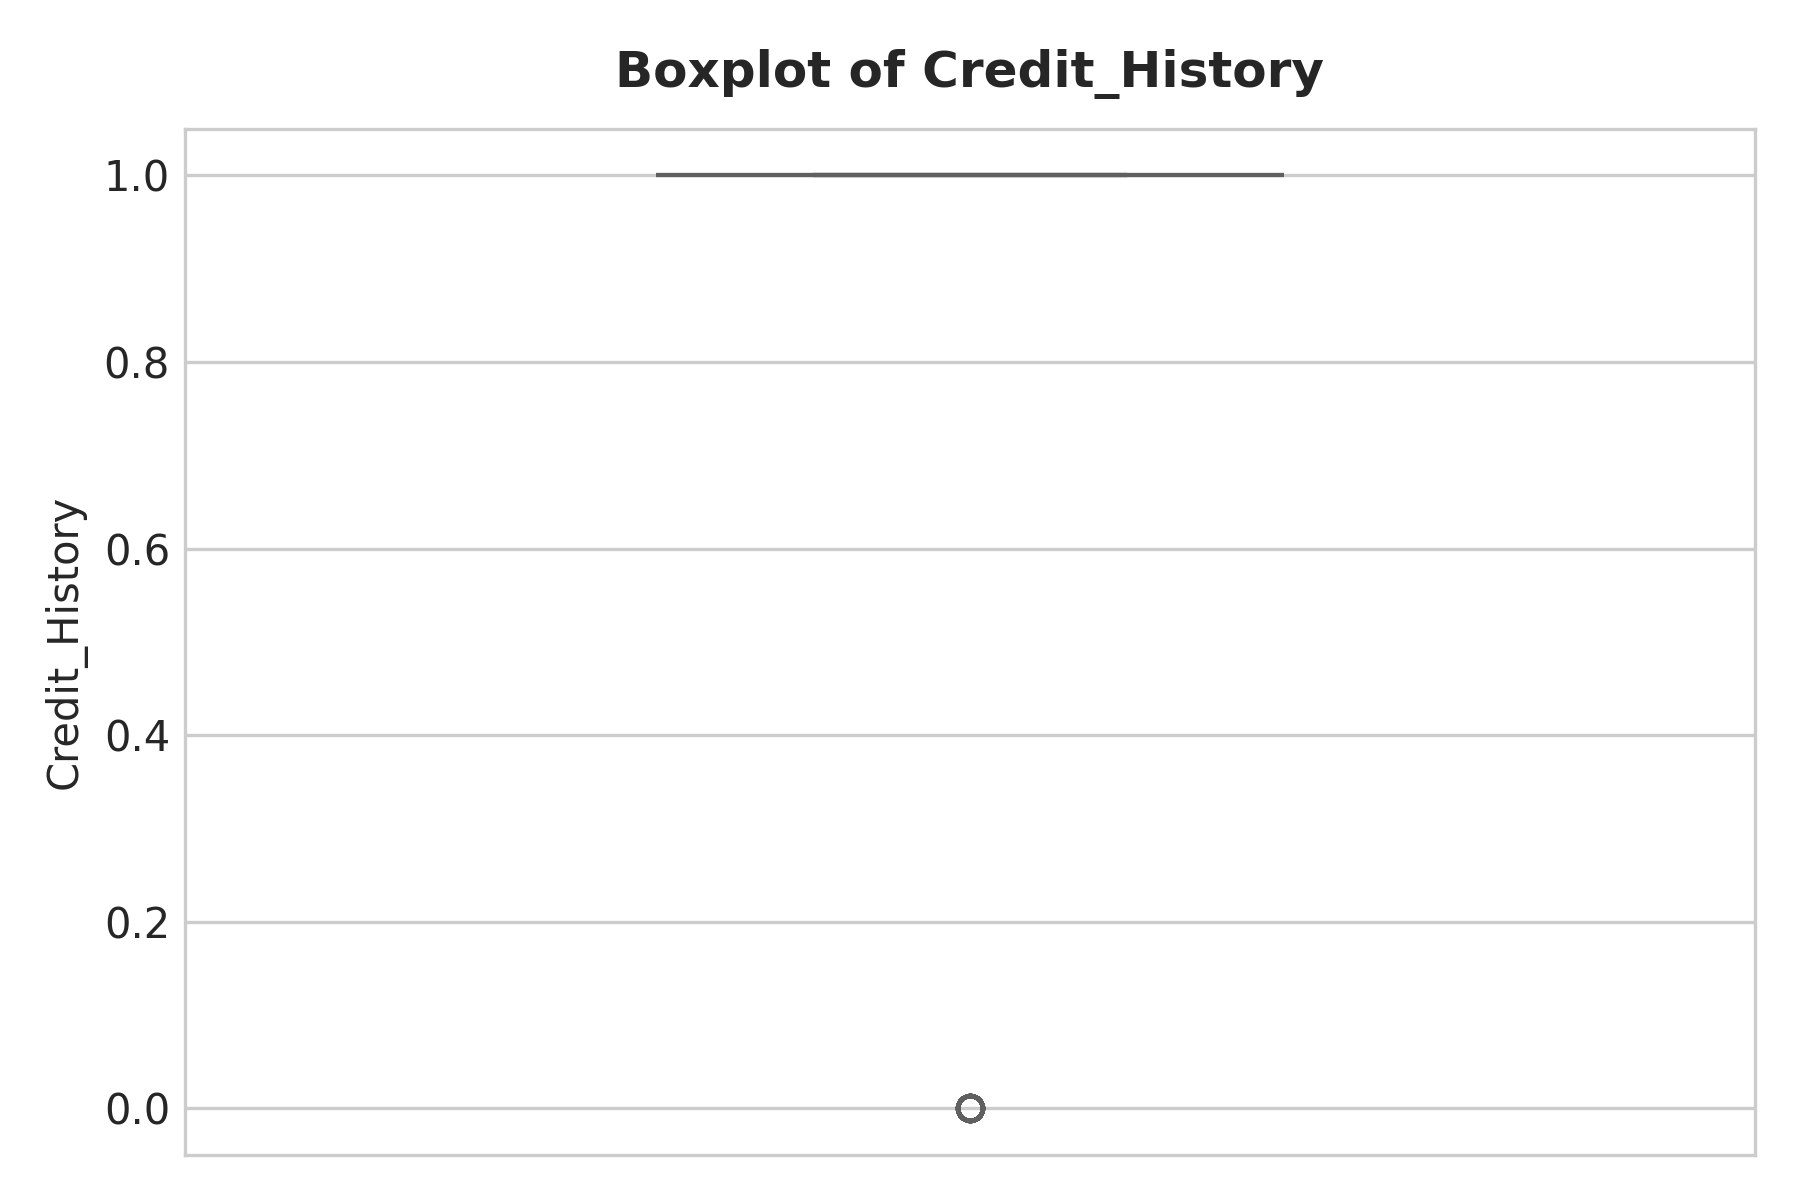
\includegraphics[width=0.75\linewidth]{figures_loan/box_Credit_History.png}
\caption{Box Plot of Credit History}
\label{fig:box_credit_history}
\end{figure}
\textbf{Inference:} The box plot compresses at 1.0 due to the high proportion of positive credit scores, reflecting discrete binary behavior.

\subsection{Kernel Density Estimation (KDE) Plots}

\begin{figure}[H]
\centering
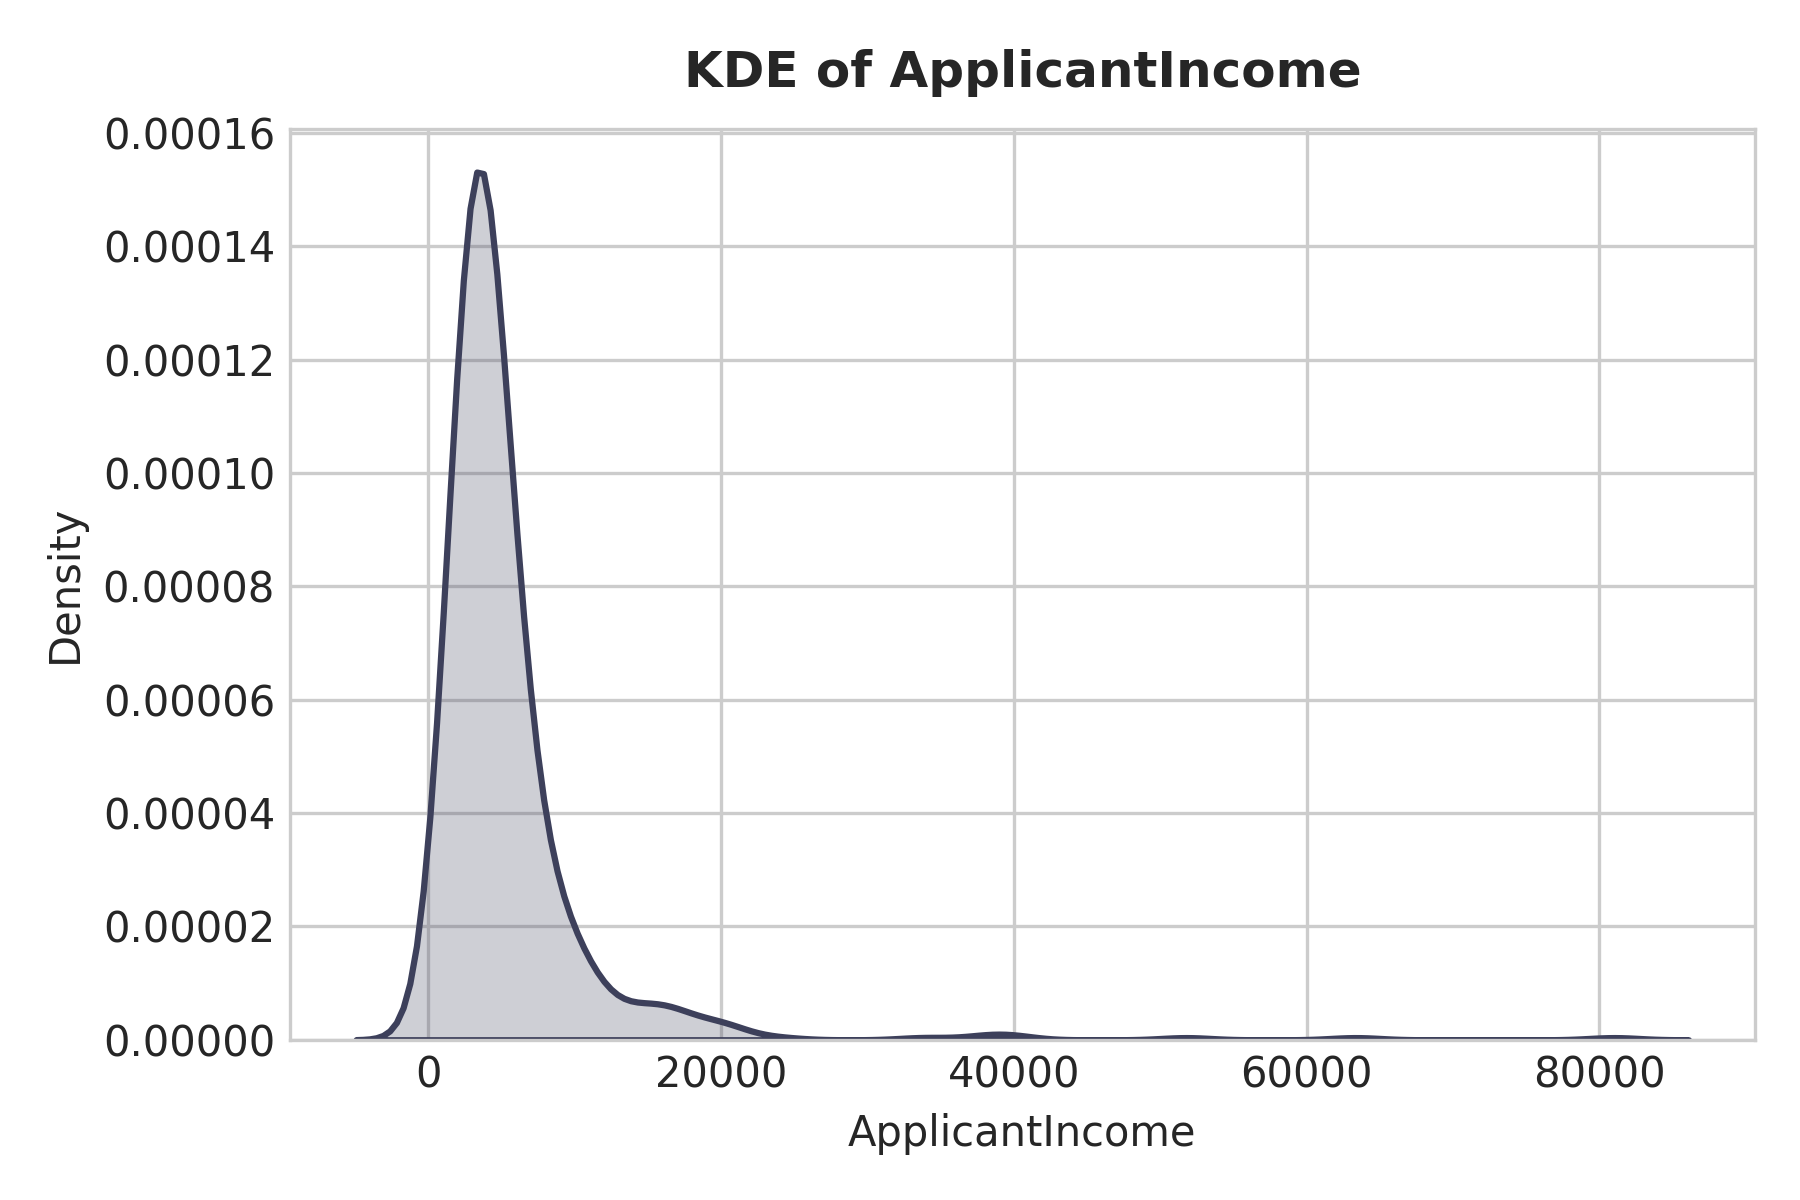
\includegraphics[width=0.75\linewidth]{figures_loan/kde_ApplicantIncome.png}
\caption{KDE of Applicant Income}
\label{fig:kde_app_income}
\end{figure}
\textbf{Inference:} The Gaussian smooth density curve highlights the single primary peak around \$3,500 with a long exponential decay toward higher income values.

\begin{figure}[H]
\centering
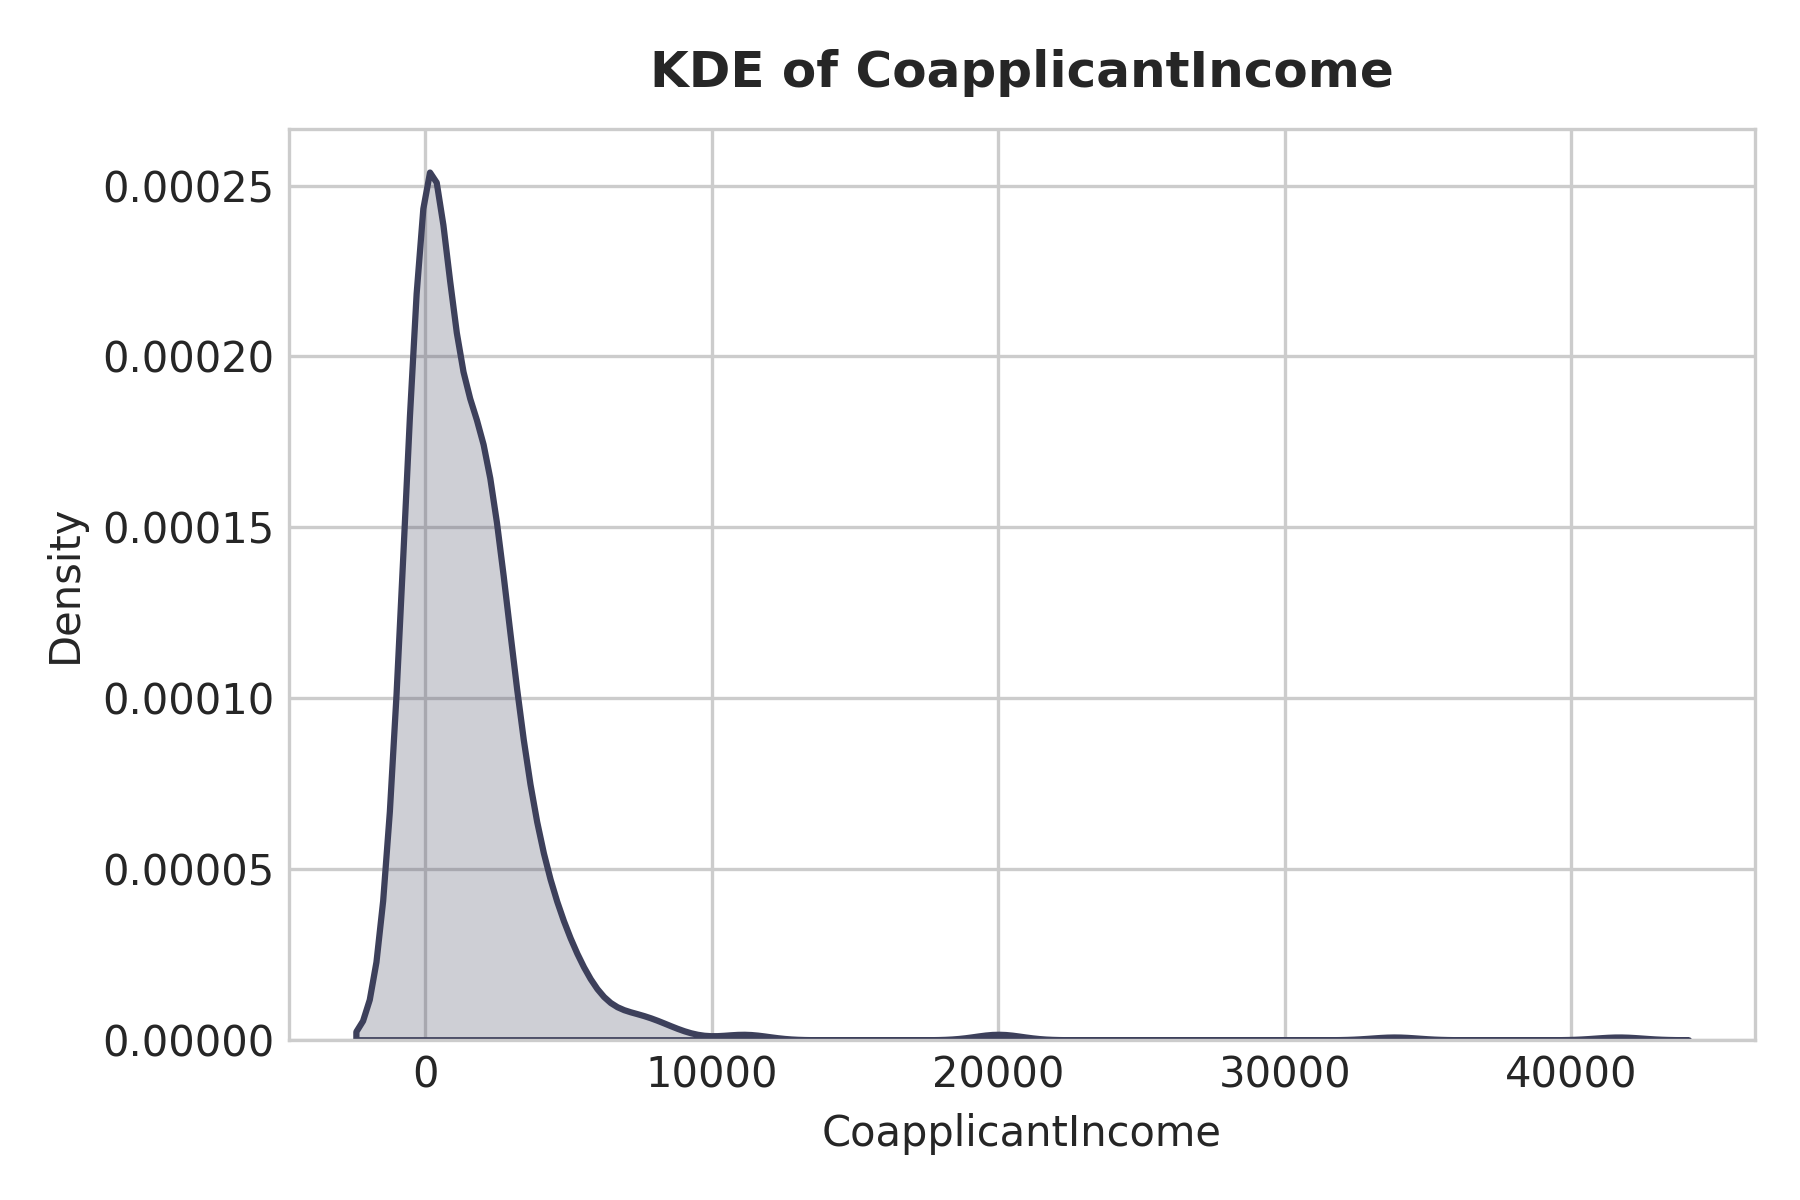
\includegraphics[width=0.75\linewidth]{figures_loan/kde_CoapplicantIncome.png}
\caption{KDE of Co-applicant Income}
\label{fig:kde_coapp_income}
\end{figure}
\textbf{Inference:} Confirms a dominant density peak near \$0 representing solo applications, followed by a smoothly decaying distribution.

\begin{figure}[H]
\centering
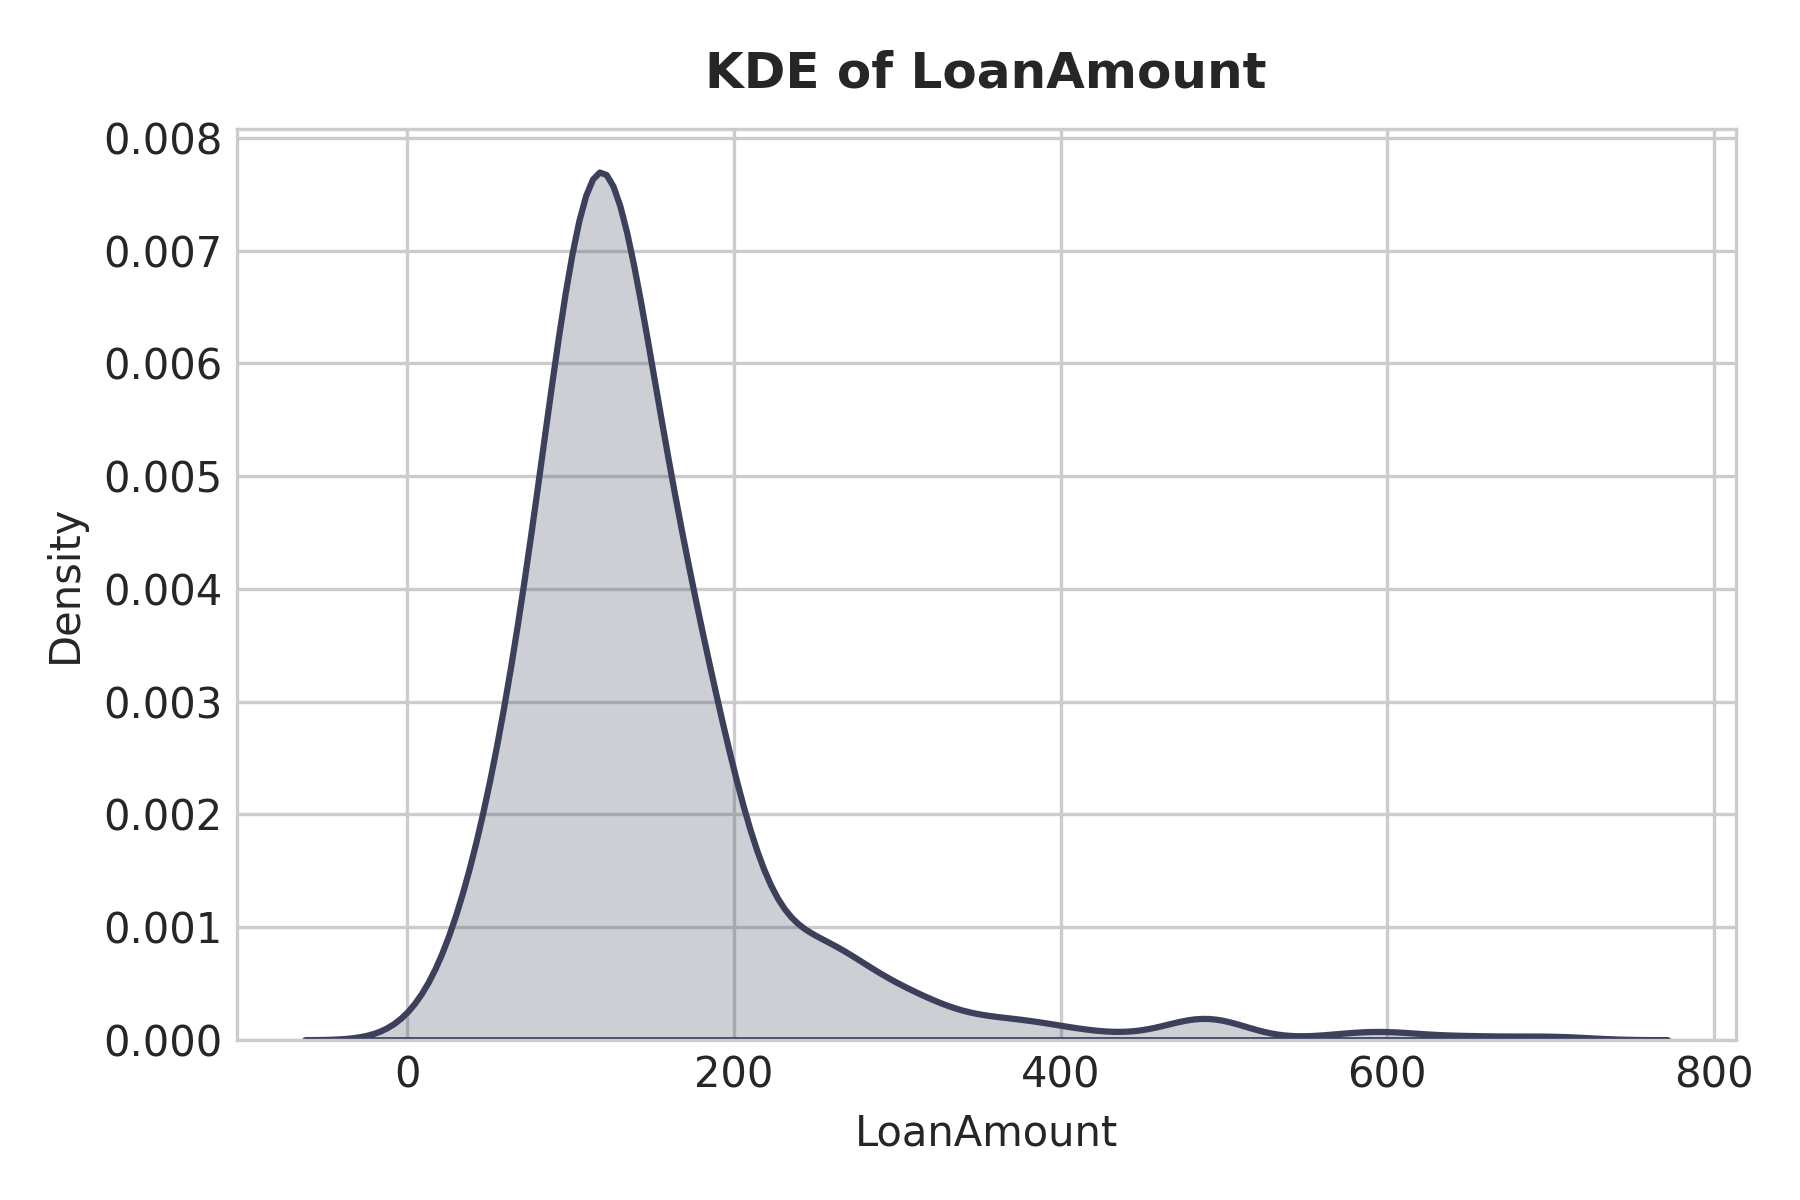
\includegraphics[width=0.75\linewidth]{figures_loan/kde_LoanAmount.png}
\caption{KDE of Loan Amount}
\label{fig:kde_loan_amount}
\end{figure}
\textbf{Inference:} The continuous density estimate displays near log-normal behavior, peaking cleanly around \$125,000.

\begin{figure}[H]
\centering
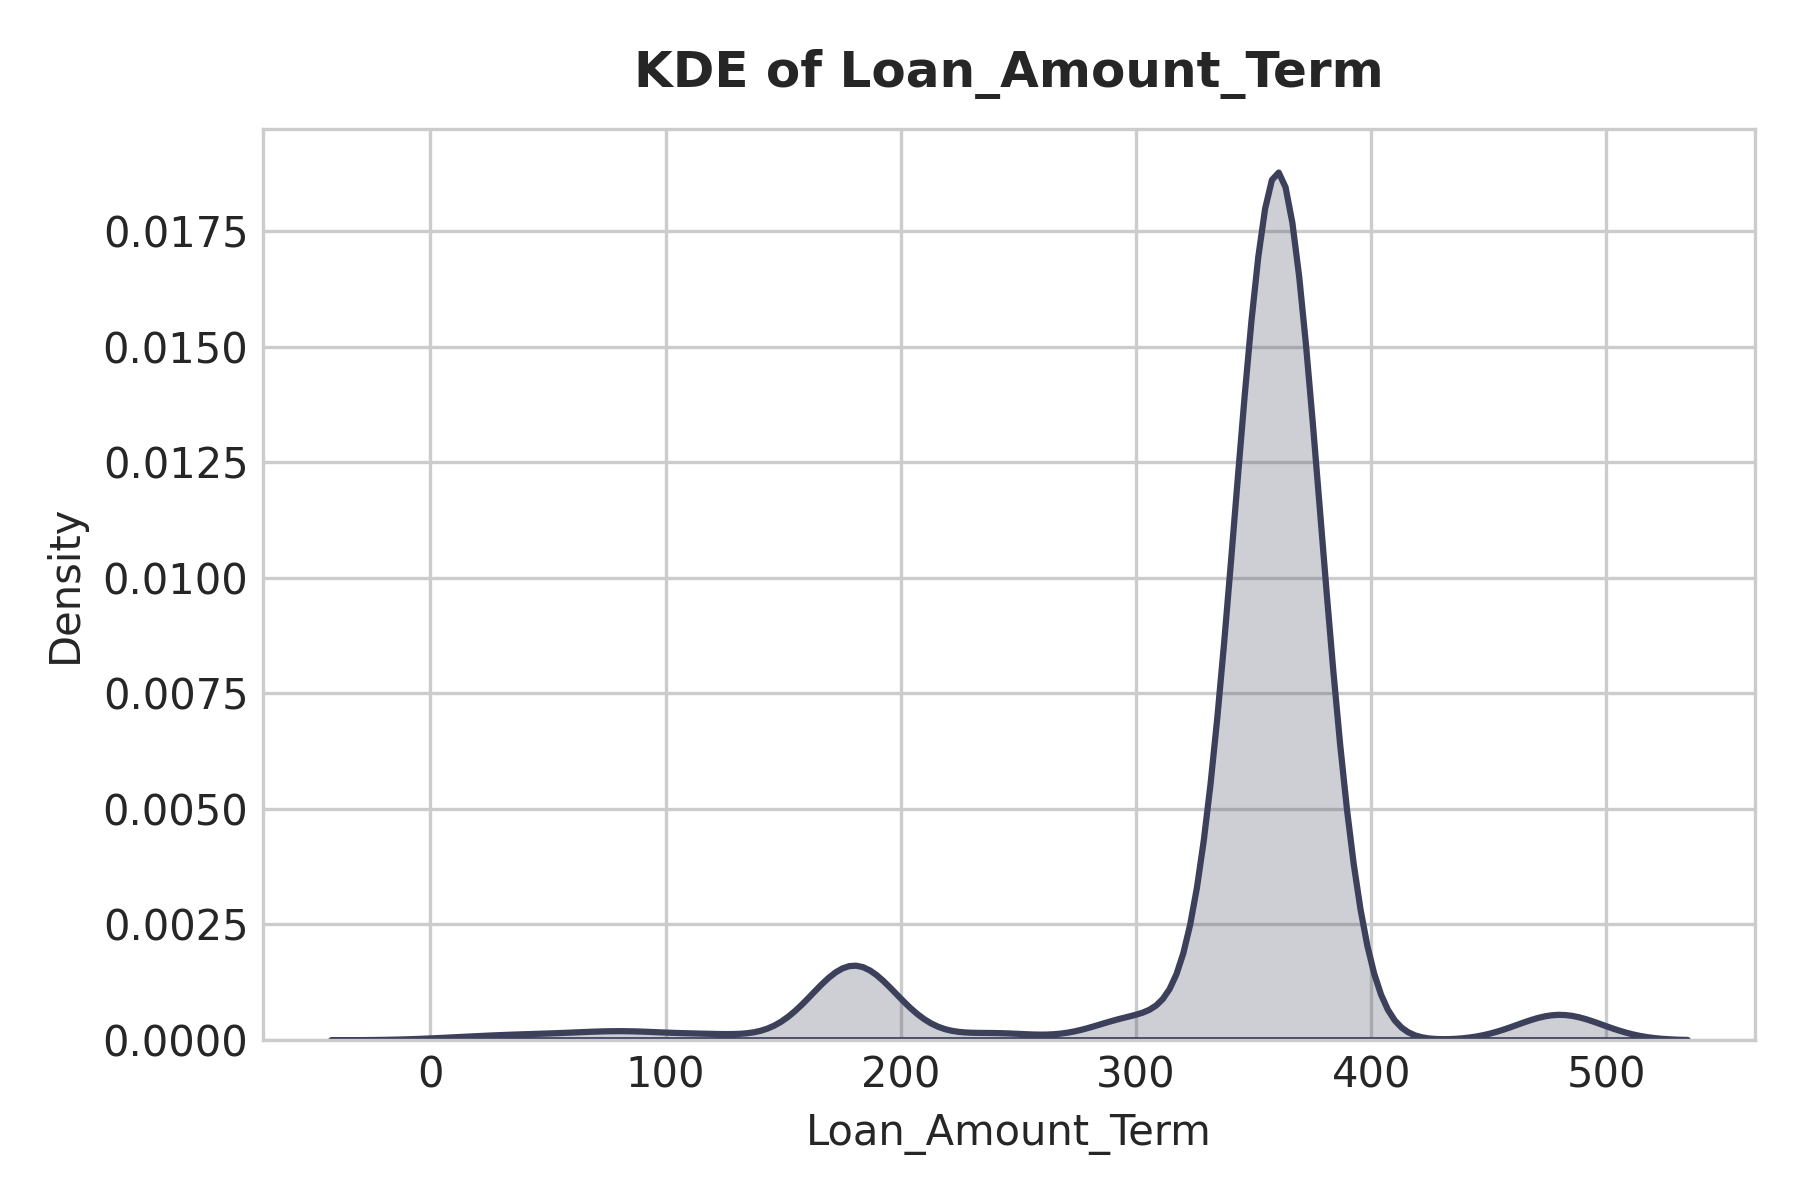
\includegraphics[width=0.75\linewidth]{figures_loan/kde_Loan_Amount_Term.png}
\caption{KDE of Loan Amount Term}
\label{fig:kde_loan_term}
\end{figure}
\textbf{Inference:} Displays an extremely narrow peak centered precisely at 360 months.

\begin{figure}[H]
\centering
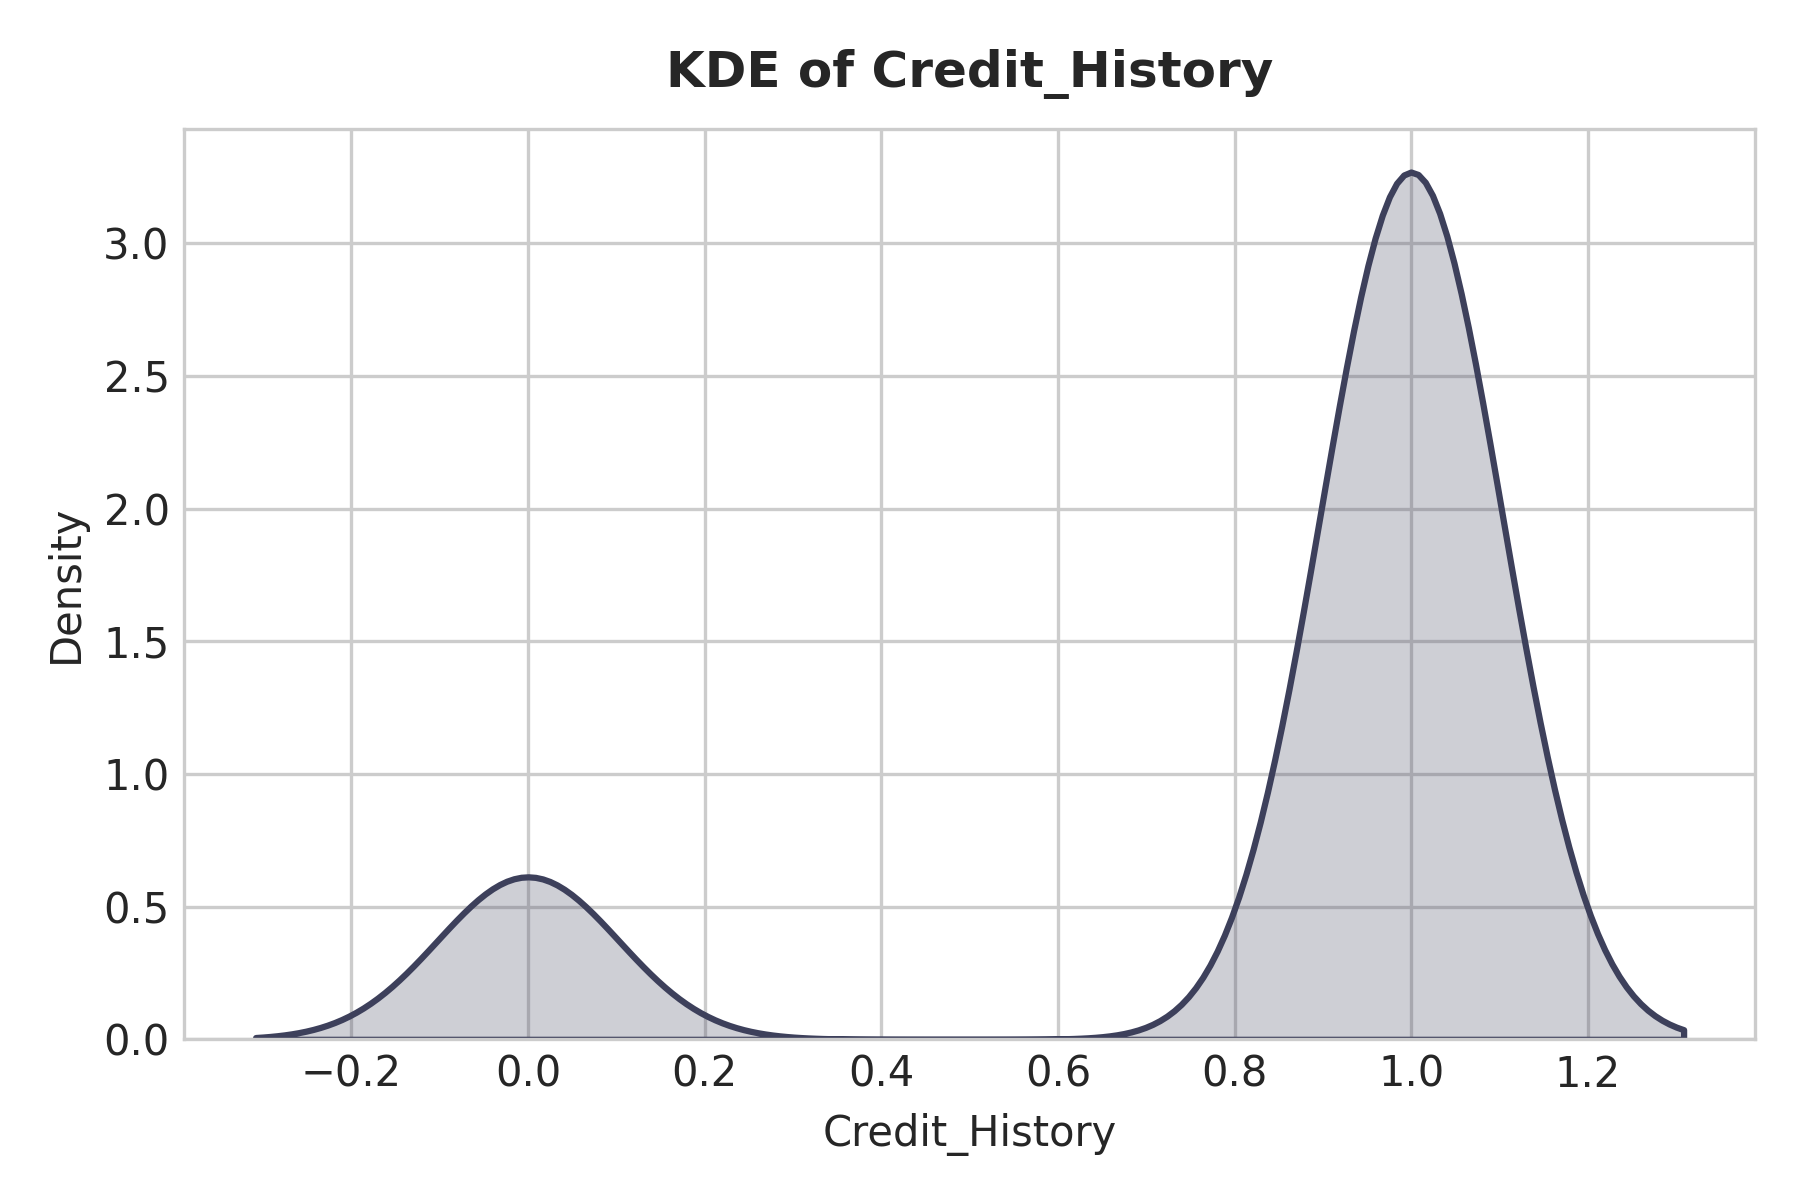
\includegraphics[width=0.75\linewidth]{figures_loan/kde_Credit_History.png}
\caption{KDE of Credit History}
\label{fig:kde_credit_history}
\end{figure}
\textbf{Inference:} Bimodal density peaks near 0.0 and 1.0 clearly illustrate the binary nature of historical credit standing.

\subsection{Count Plots of Categorical Features}

\begin{figure}[H]
\centering
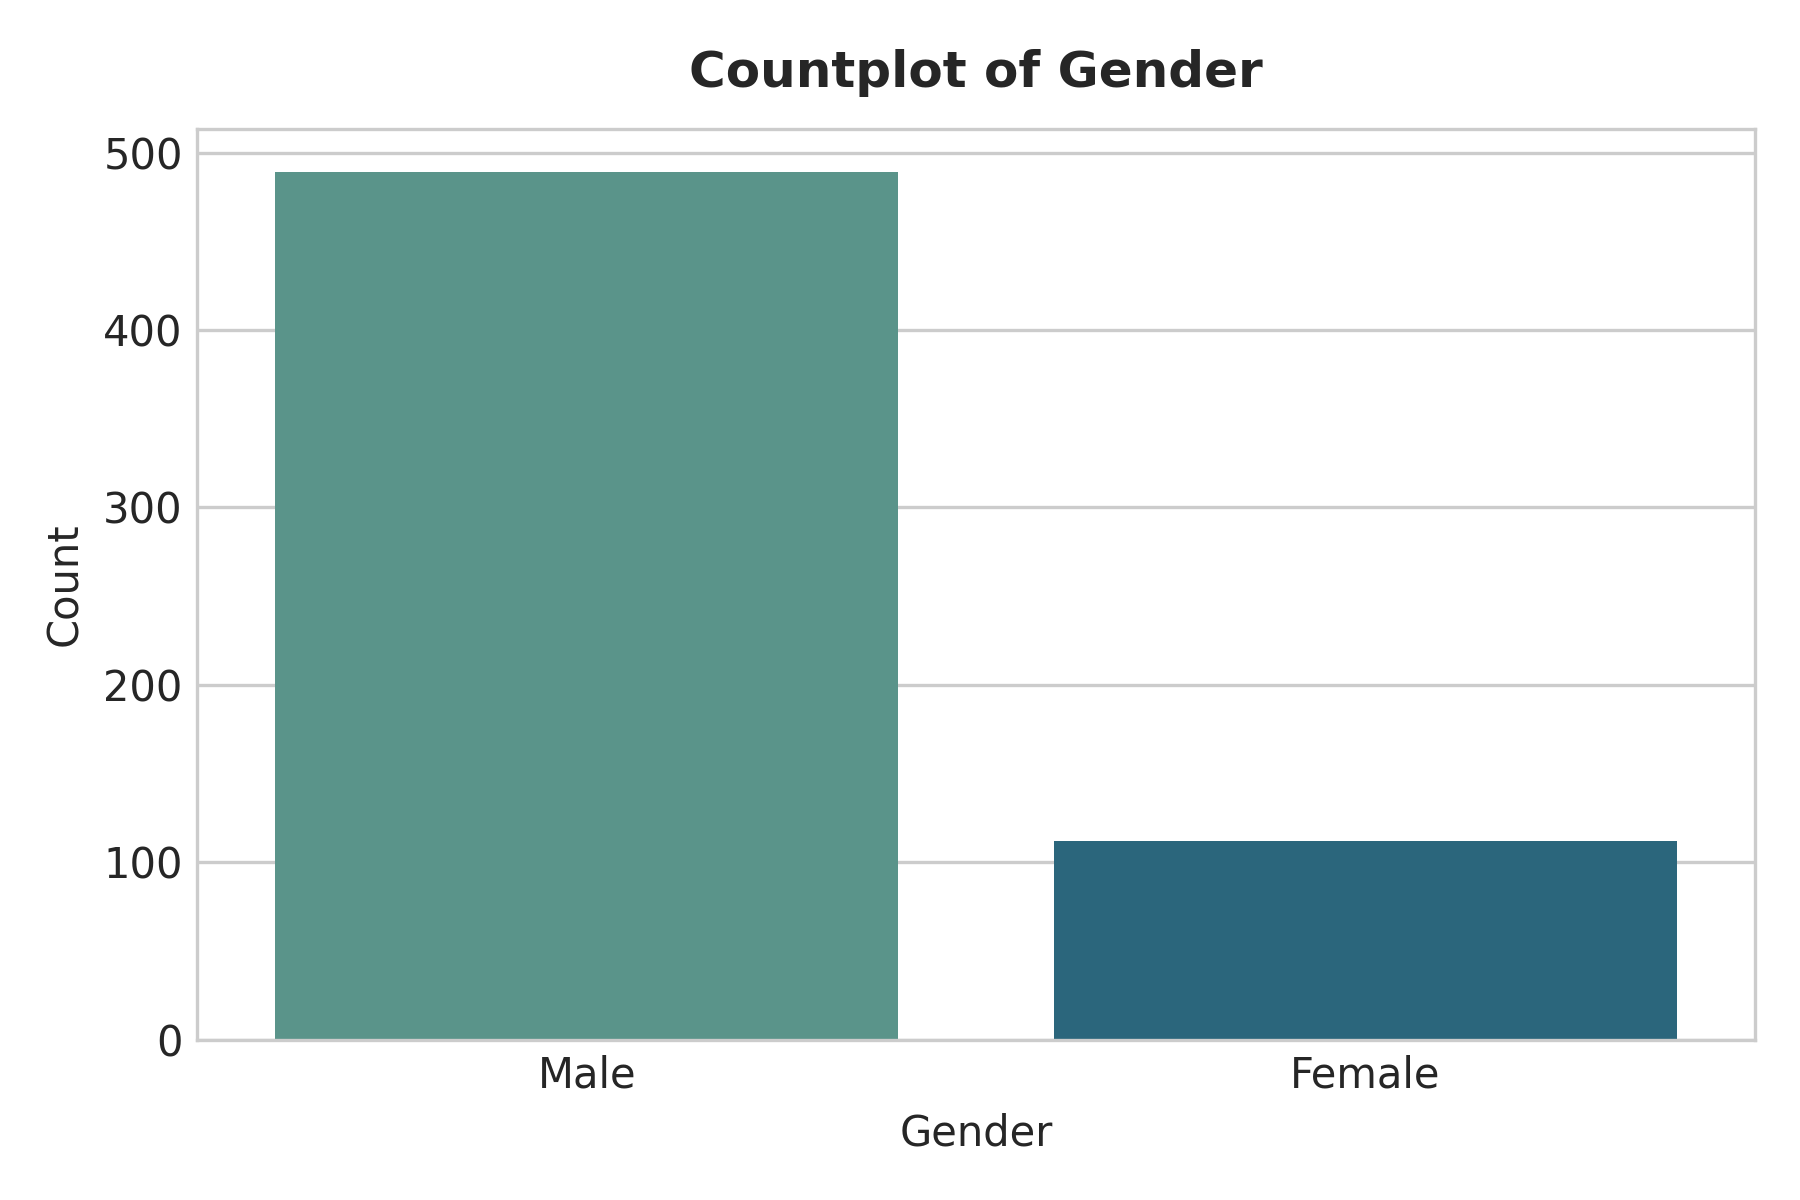
\includegraphics[width=0.75\linewidth]{figures_loan/count_Gender.png}
\caption{Count Plot of Gender}
\label{fig:count_gender}
\end{figure}
\textbf{Inference:} Male applicants comprise over 80\% of the records, highlighting gender imbalance within the historical sampling pool.

\begin{figure}[H]
\centering
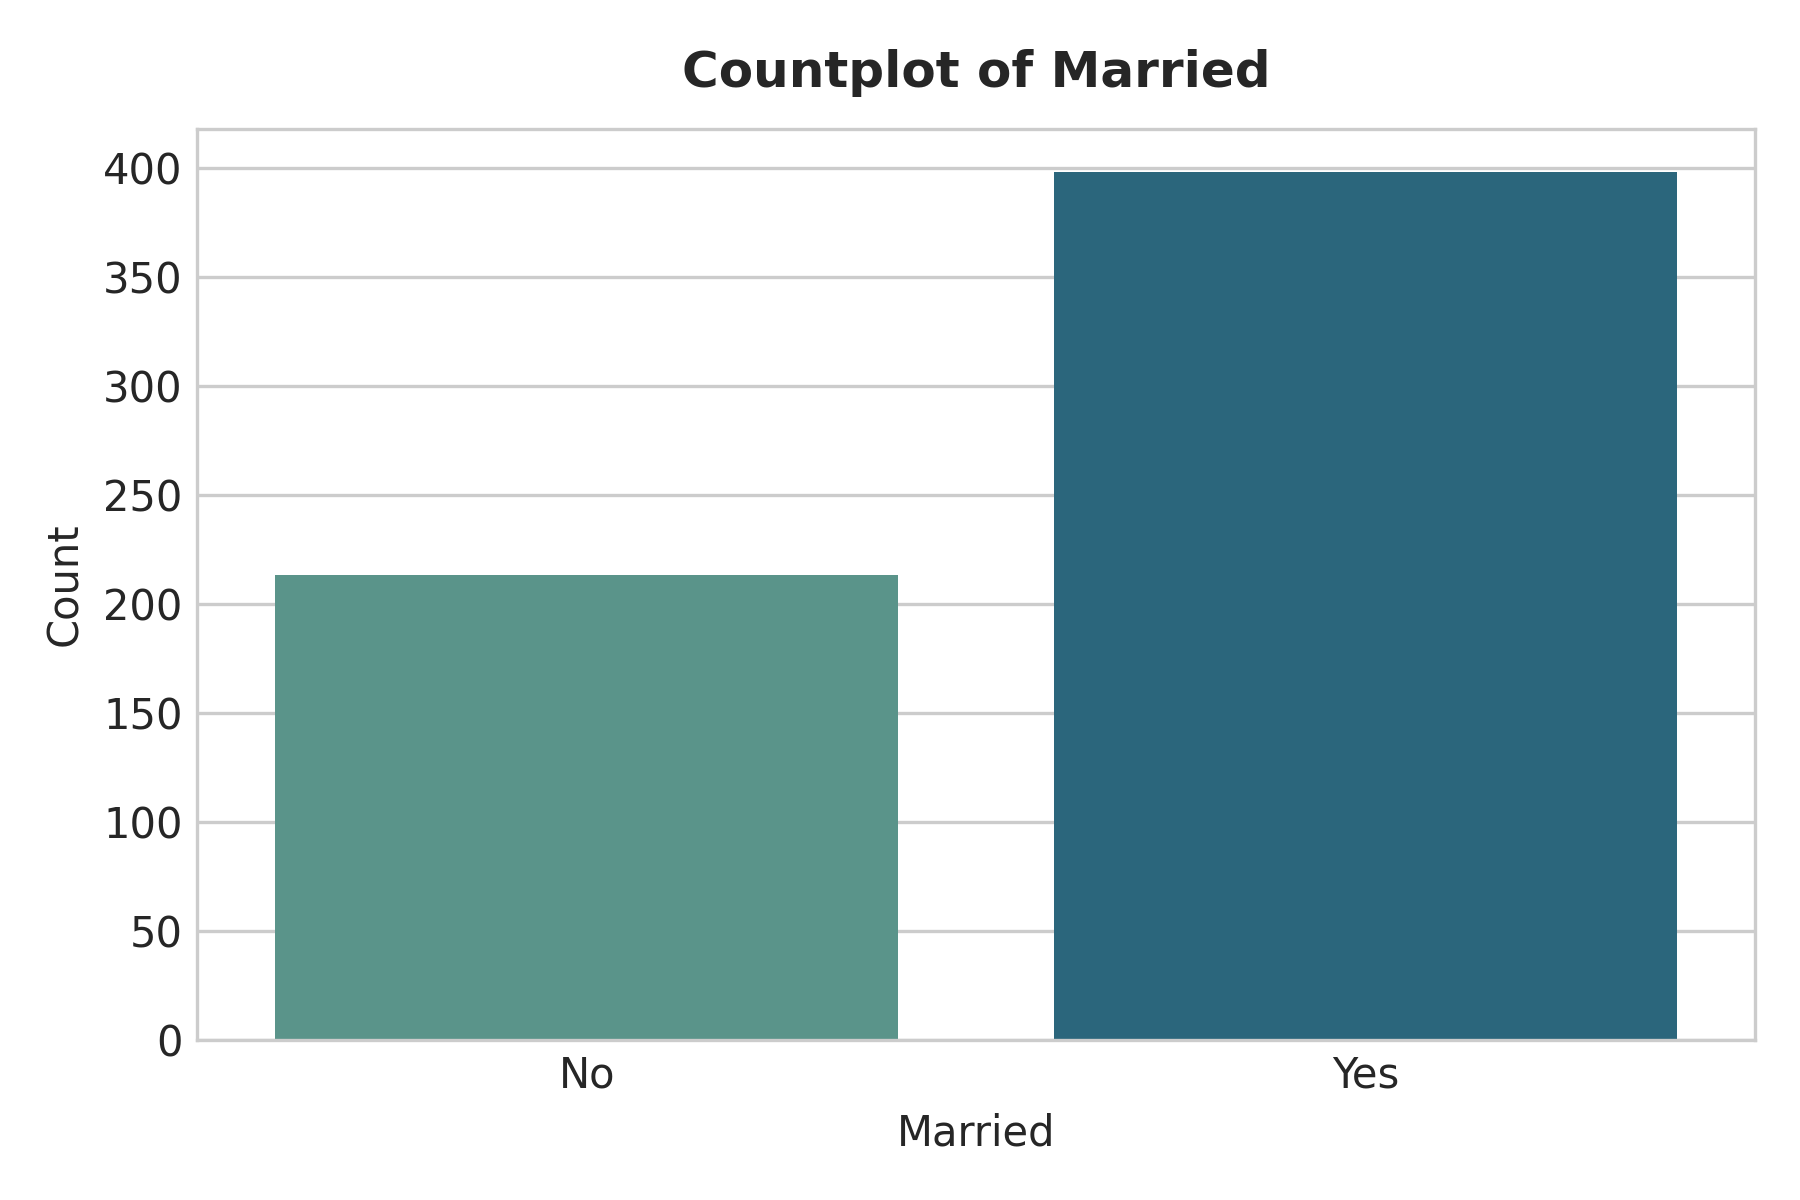
\includegraphics[width=0.75\linewidth]{figures_loan/count_Married.png}
\caption{Count Plot of Married}
\label{fig:count_married}
\end{figure}
\textbf{Inference:} Married individuals account for roughly two-thirds of total applications, reflecting joint credit applications.

\begin{figure}[H]
\centering
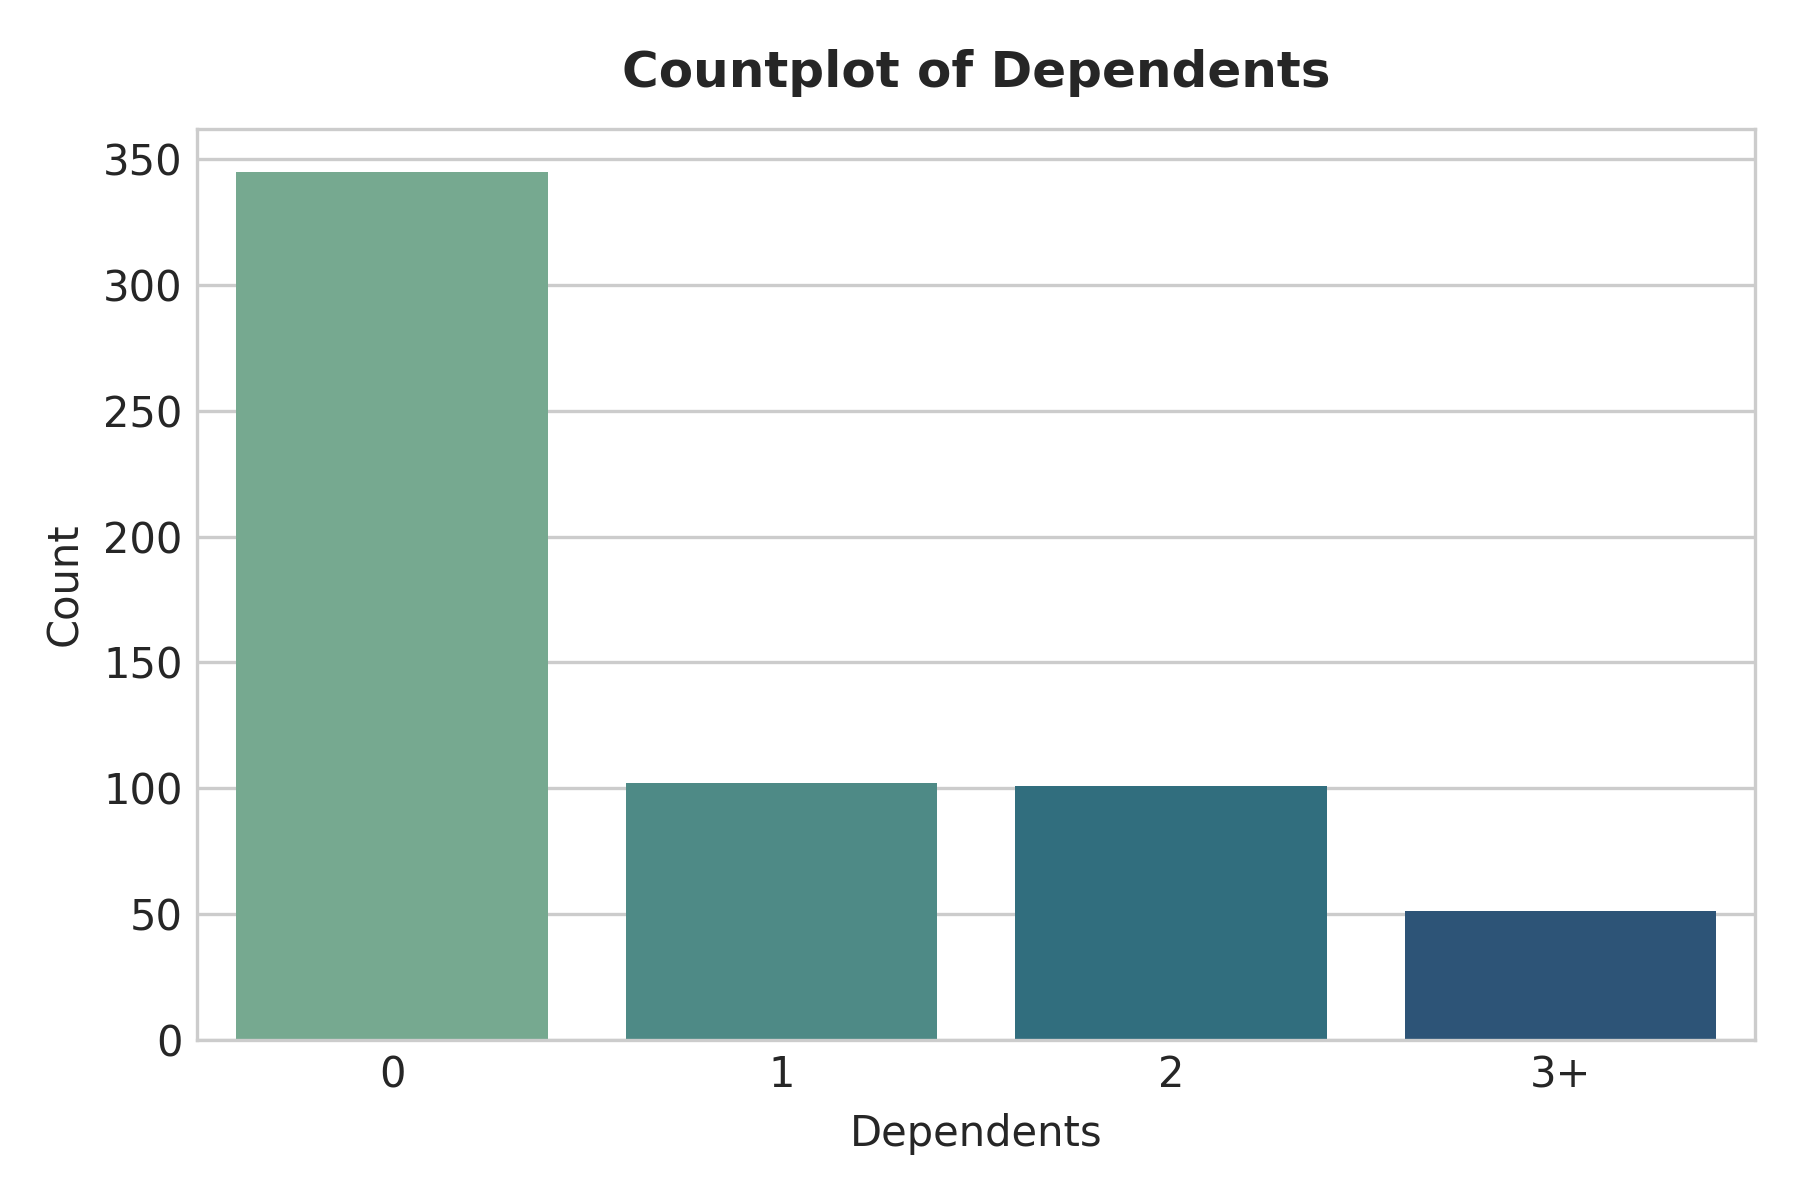
\includegraphics[width=0.75\linewidth]{figures_loan/count_Dependents.png}
\caption{Count Plot of Dependents}
\label{fig:count_dependents}
\end{figure}
\textbf{Inference:} Applicants with 0 dependents form the largest demographic group, followed by 1, 2, and 3+ dependents in descending frequency.

\begin{figure}[H]
\centering
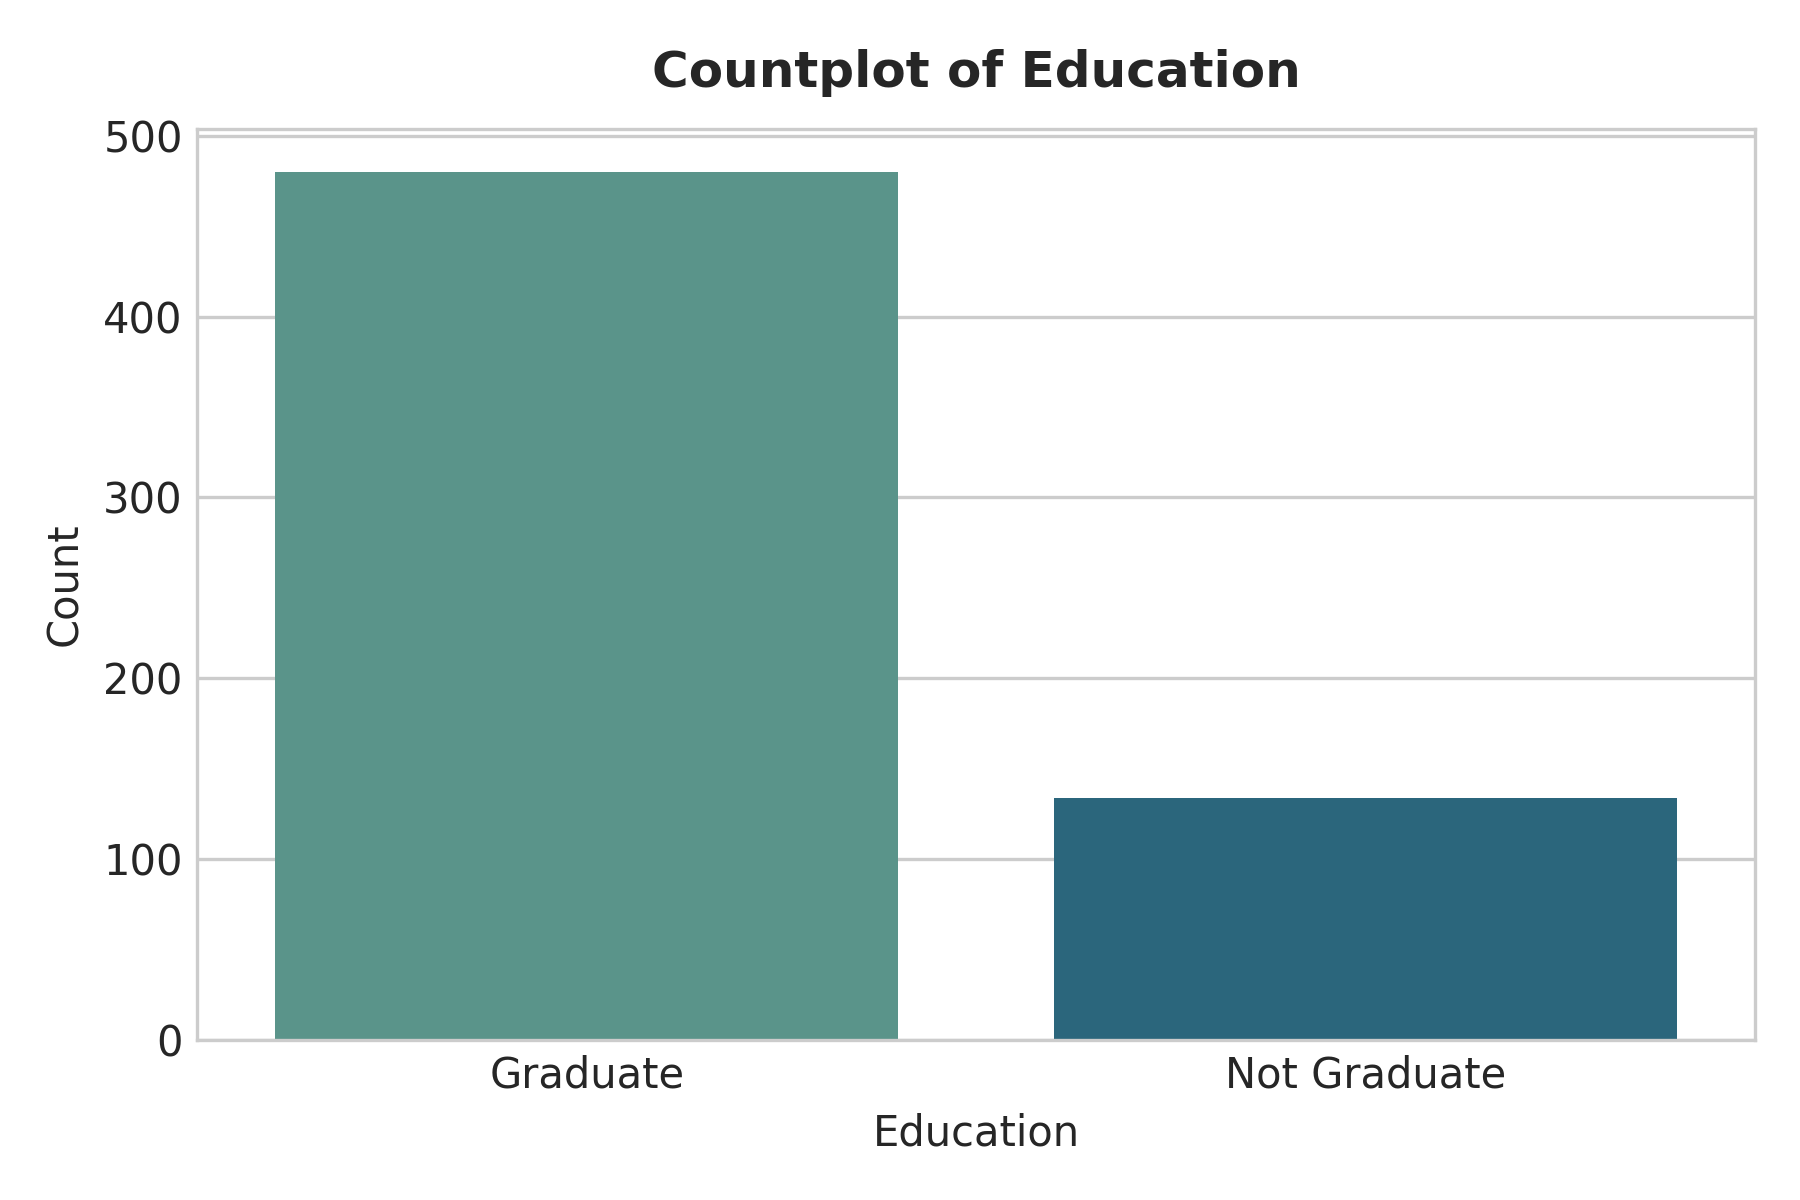
\includegraphics[width=0.75\linewidth]{figures_loan/count_Education.png}
\caption{Count Plot of Education}
\label{fig:count_education}
\end{figure}
\textbf{Inference:} Graduates constitute approximately 78\% of total applicants compared to non-graduates.

\begin{figure}[H]
\centering
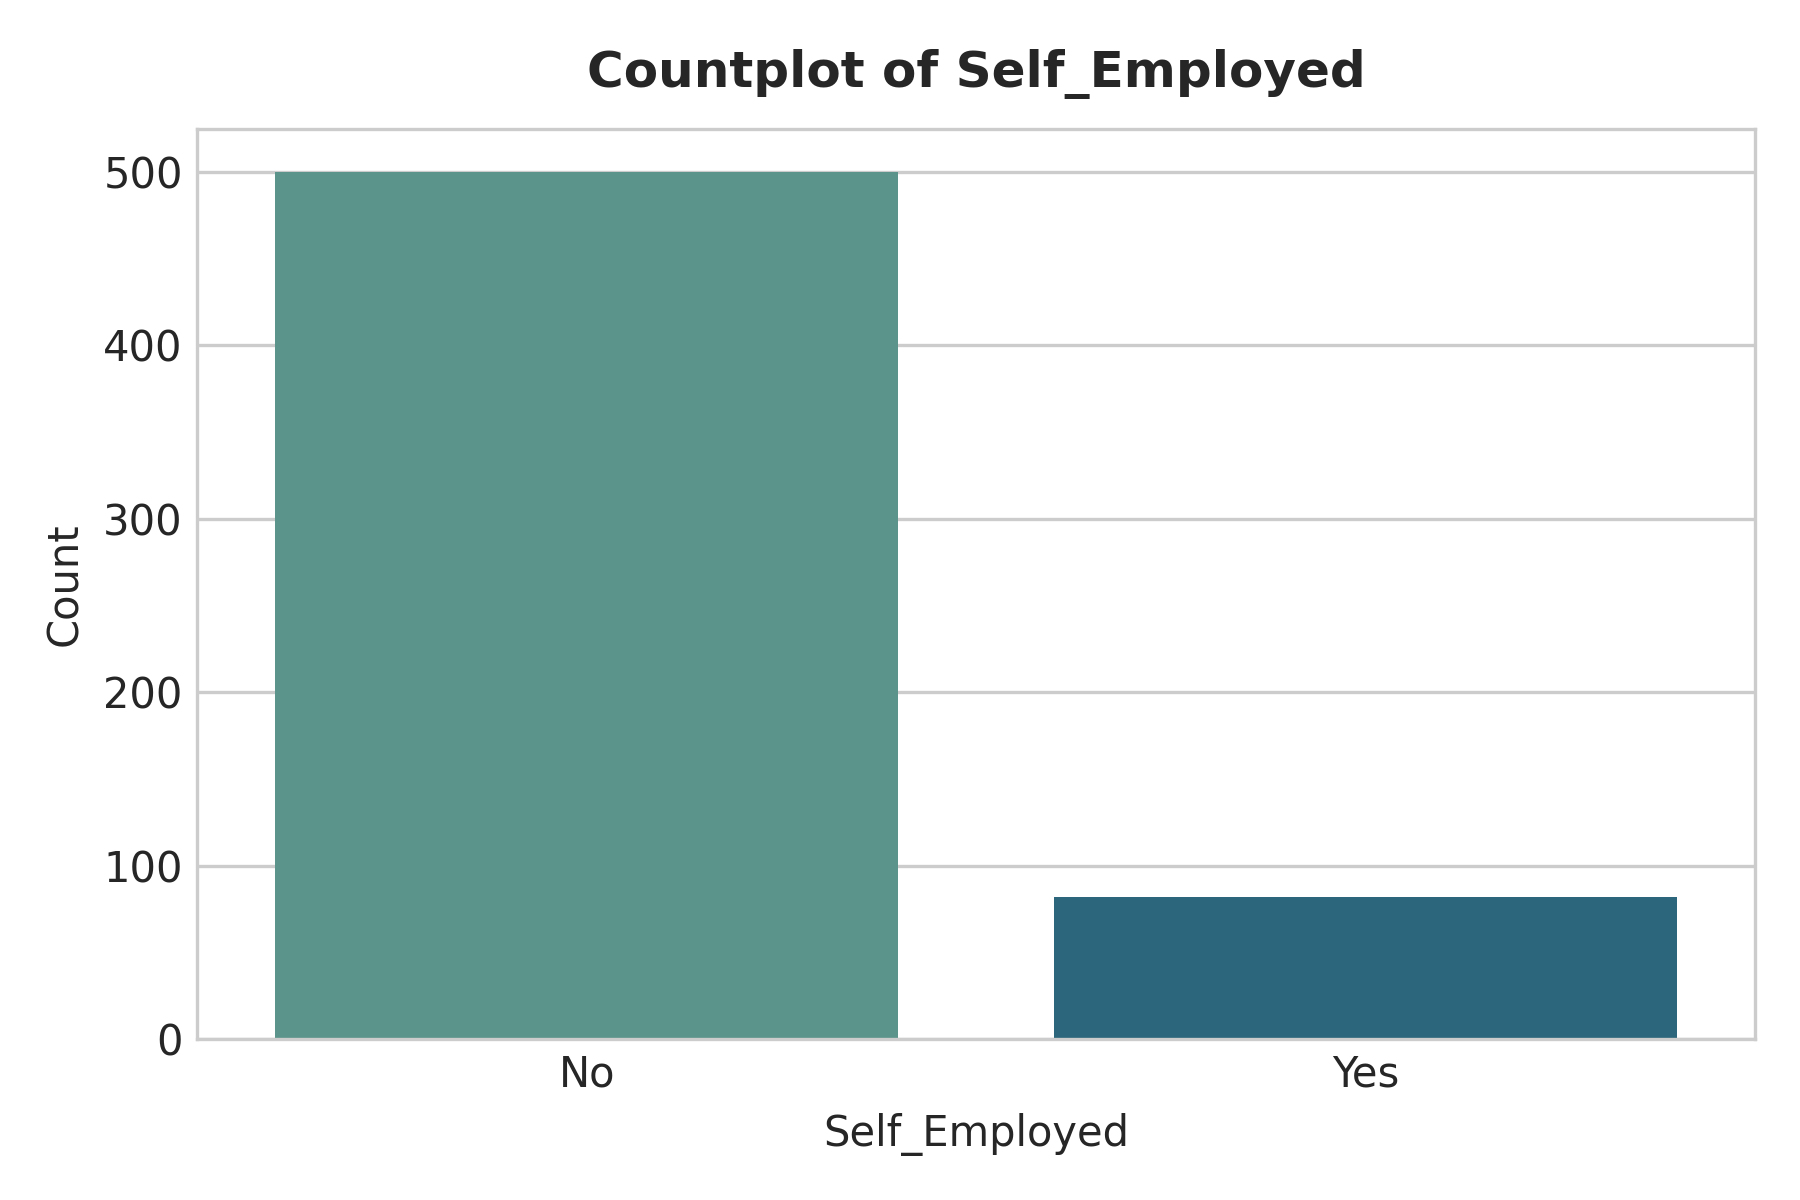
\includegraphics[width=0.75\linewidth]{figures_loan/count_Self_Employed.png}
\caption{Count Plot of Self Employed}
\label{fig:count_self_employed}
\end{figure}
\textbf{Inference:} Self-employed individuals represent only 14\% of applicants, with the majority being salaried employees.

\begin{figure}[H]
\centering
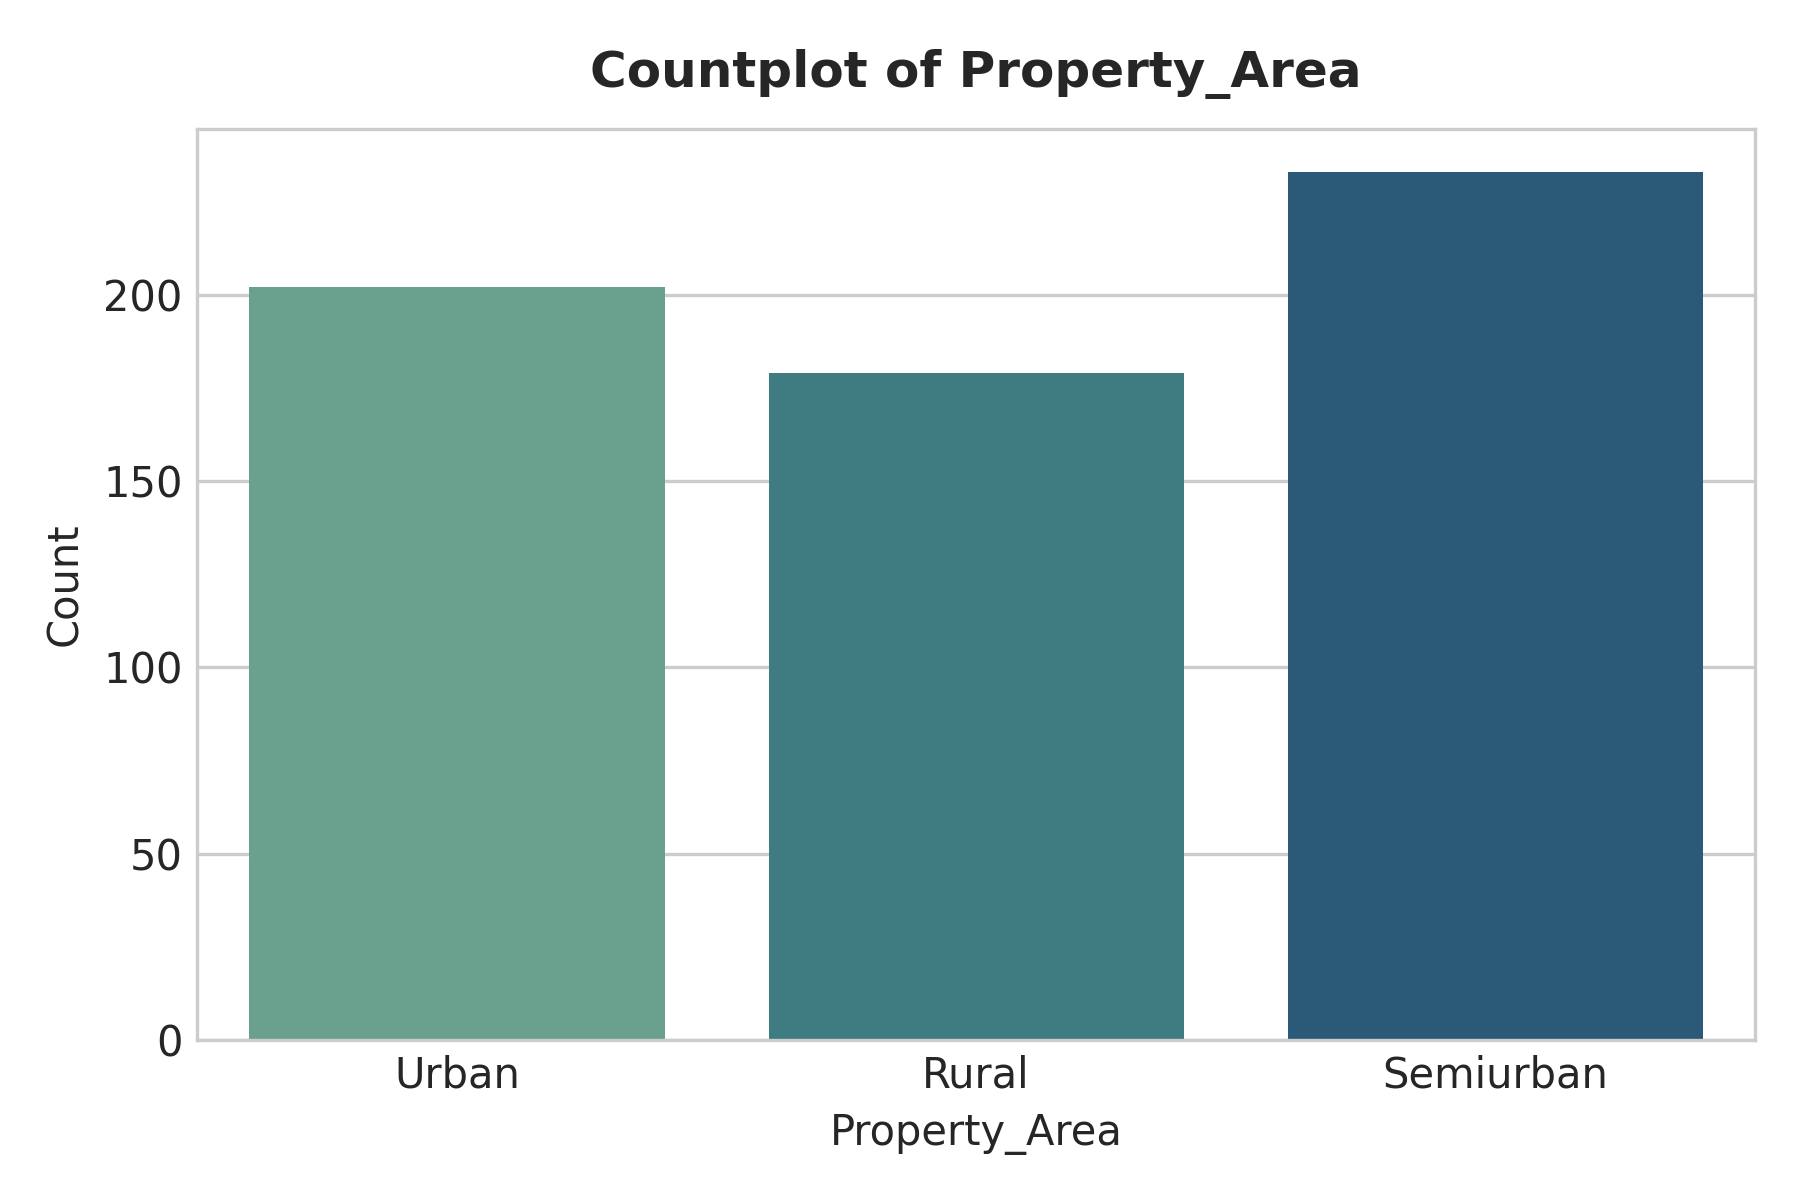
\includegraphics[width=0.75\linewidth]{figures_loan/count_Property_Area.png}
\caption{Count Plot of Property Area}
\label{fig:count_property}
\end{figure}
\textbf{Inference:} Property locations are fairly balanced across categories, with Semiurban slightly exceeding Urban and Rural areas.

\begin{figure}[H]
\centering
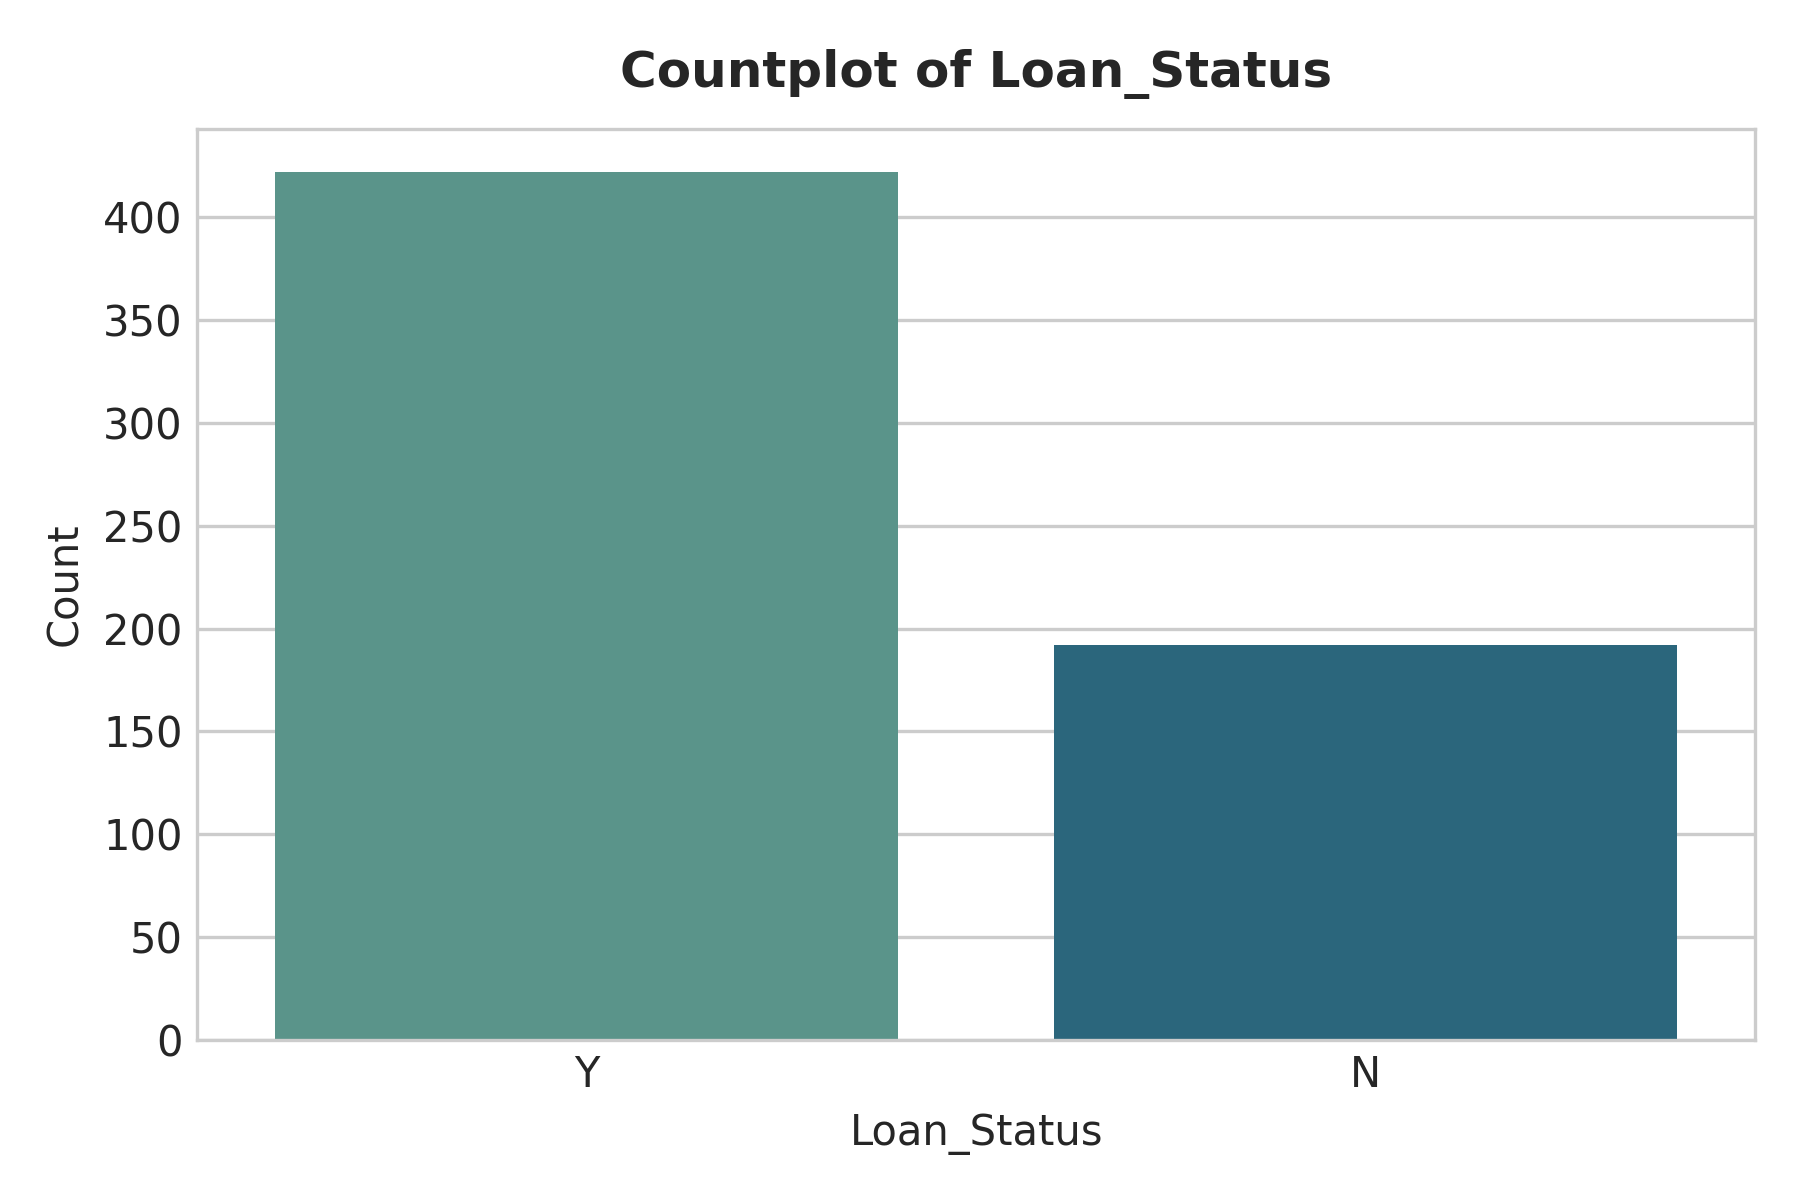
\includegraphics[width=0.75\linewidth]{figures_loan/count_Loan_Status.png}
\caption{Count Plot of Loan Status}
\label{fig:count_status}
\end{figure}
\textbf{Inference:} Approximately 69\% of loan applications in the dataset were approved (Y), while 31\% were rejected (N).

\subsection{Correlation Heatmap of Numerical Features}

\begin{figure}[H]
\centering

\includegraphics[width=0.75\linewidth]{figures_loan/correlation_heatmap.png}
\caption{Correlation Heatmap}
\label{fig:correlation_heatmap}
\end{figure}
\textbf{Inference:} A moderate positive linear correlation ($r = 0.57$) exists between \texttt{ApplicantIncome} and \texttt{LoanAmount}, demonstrating that higher earnings translate to larger requested loans. Other numerical pairs show weak linear dependencies.

\subsection{Pairwise Scatter Matrix (Pair Plot)}

\begin{figure}[H]
\centering

\includegraphics[width=0.75\linewidth]{figures_loan/pairplot.png}
\caption{Pair Plot of Features}
\label{fig:pairplot}
\end{figure}
\textbf{Inference:} The scatter matrix highlights bivariate feature interactions alongside diagonal marginal distributions. The upward linear trend between primary income and loan amount is evident across the scatter grid.

\subsection{Bivariate Scatter Plots}

\begin{figure}[H]
\centering
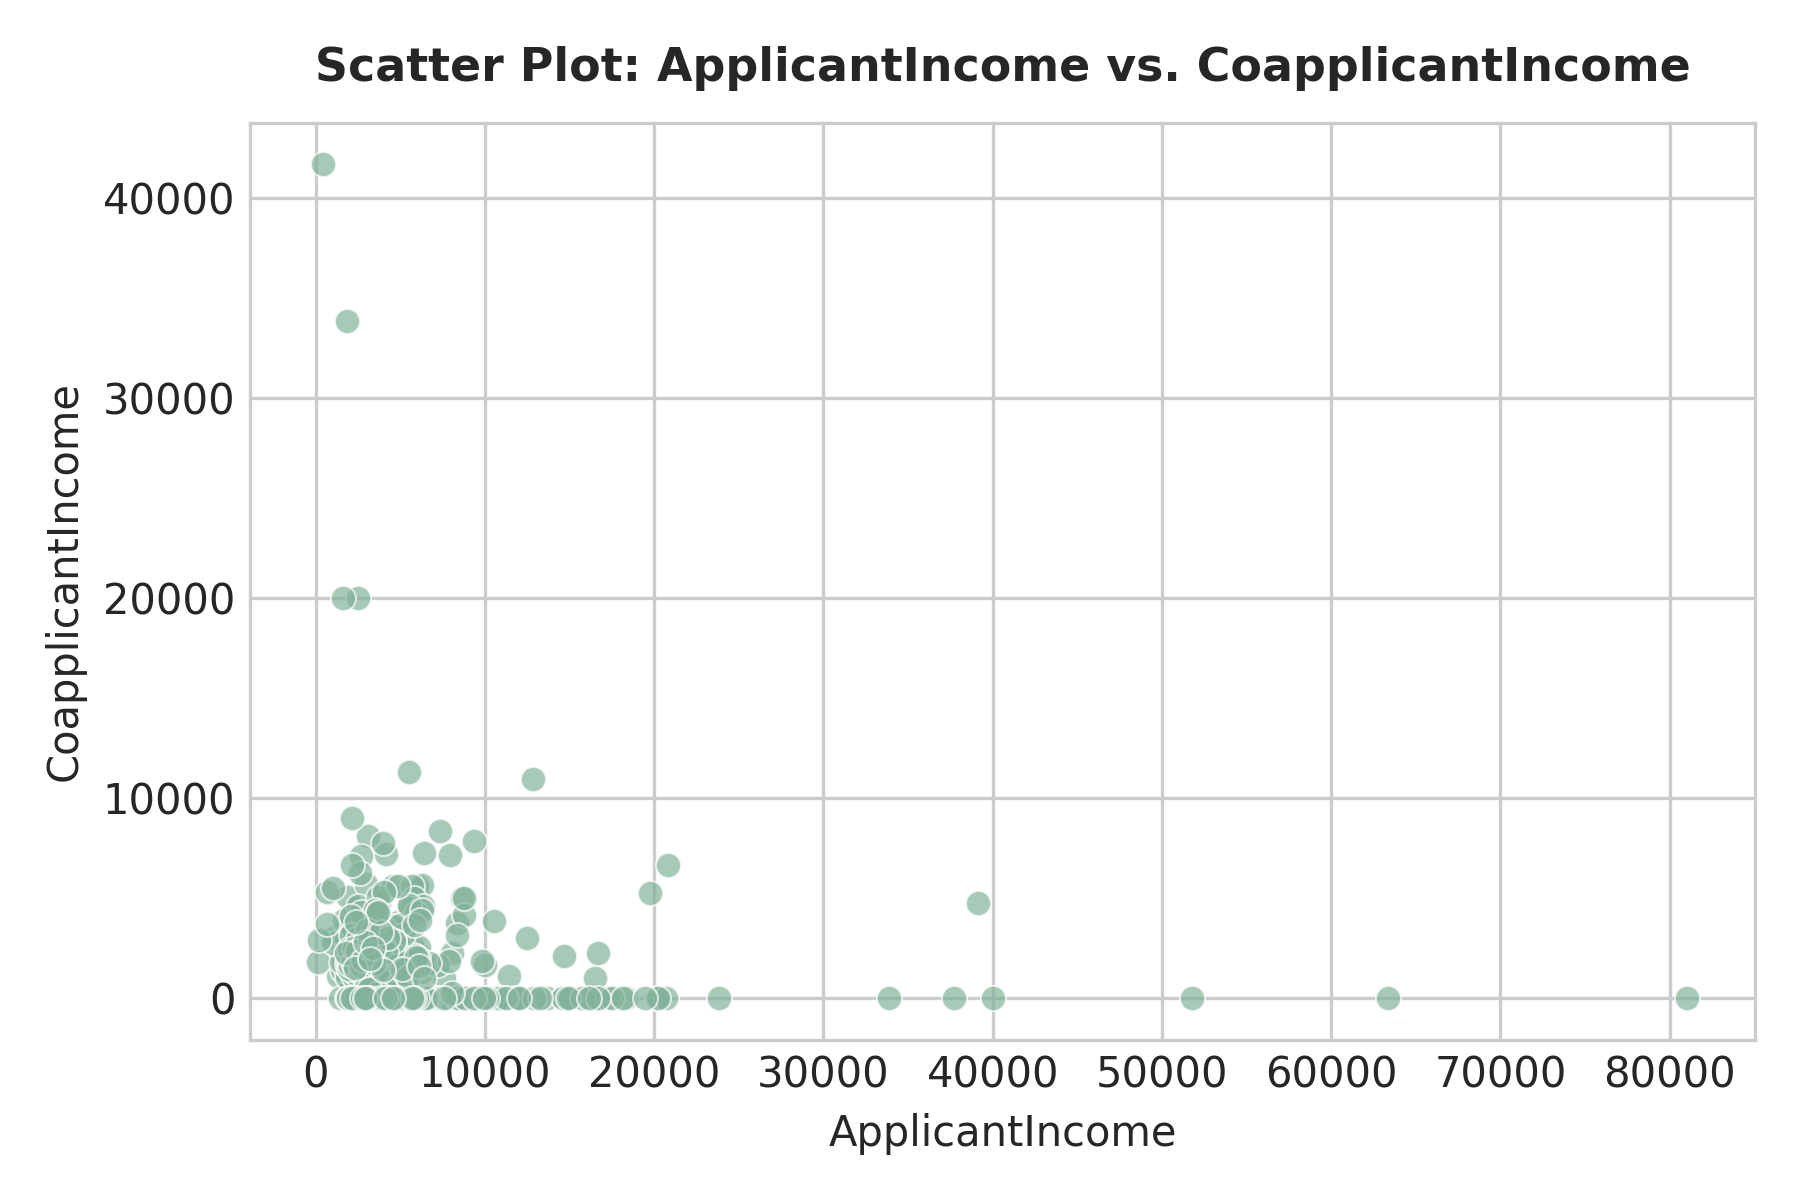
\includegraphics[width=0.75\linewidth]{figures_loan/scatter_ApplicantIncome_vs_CoapplicantIncome.png}
\caption{Scatter Plot: Applicant Income vs. Co-applicant Income}
\label{fig:scatter_app_coapp}
\end{figure}
\textbf{Inference:} Data points cluster near the origin, indicating no linear dependency between primary and secondary applicant incomes.

\begin{figure}[H]
\centering
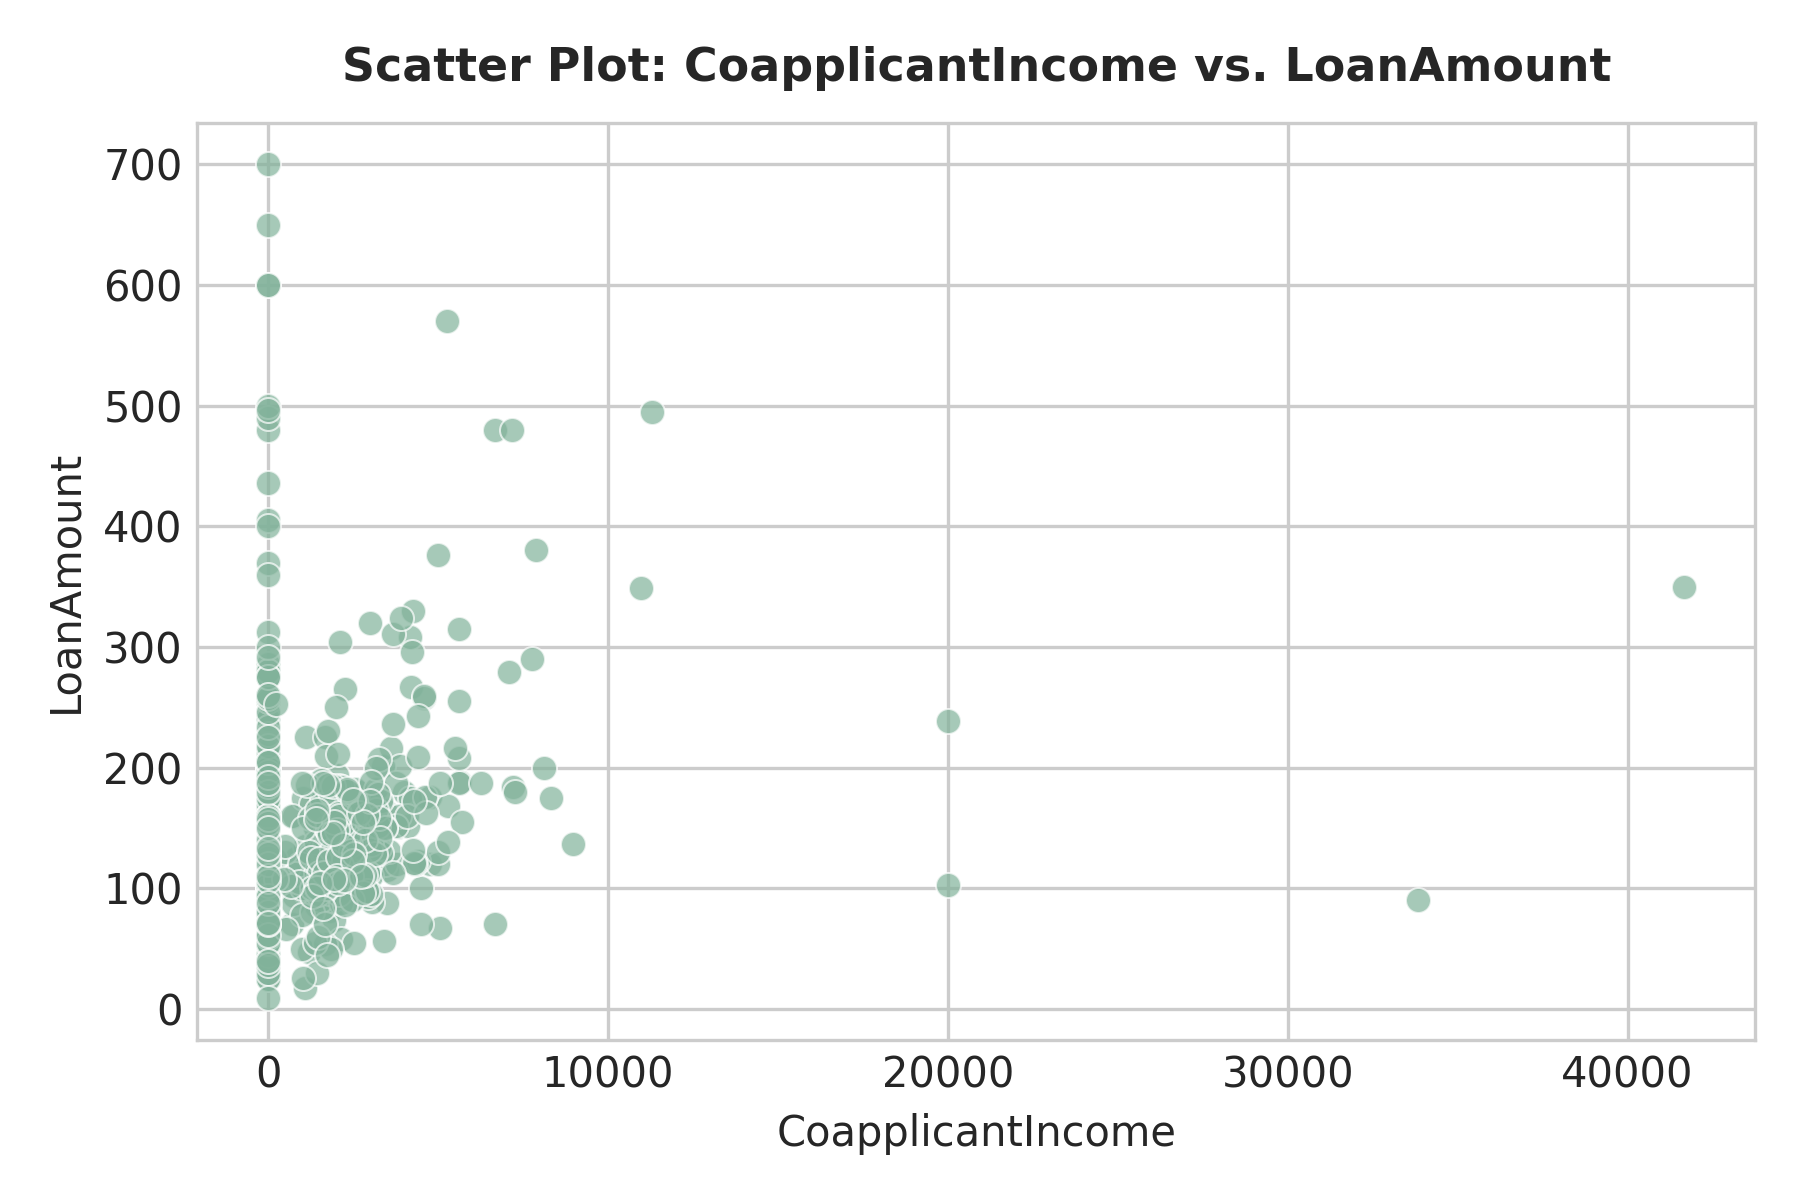
\includegraphics[width=0.75\linewidth]{figures_loan/scatter_CoapplicantIncome_vs_LoanAmount.png}
\caption{Scatter Plot: Co-applicant Income vs. Loan Amount}
\label{fig:scatter_coapp_loan}
\end{figure}
\textbf{Inference:} Displays a weak positive association ($r = 0.19$) with substantial dispersion across income levels.

\begin{figure}[H]
\centering
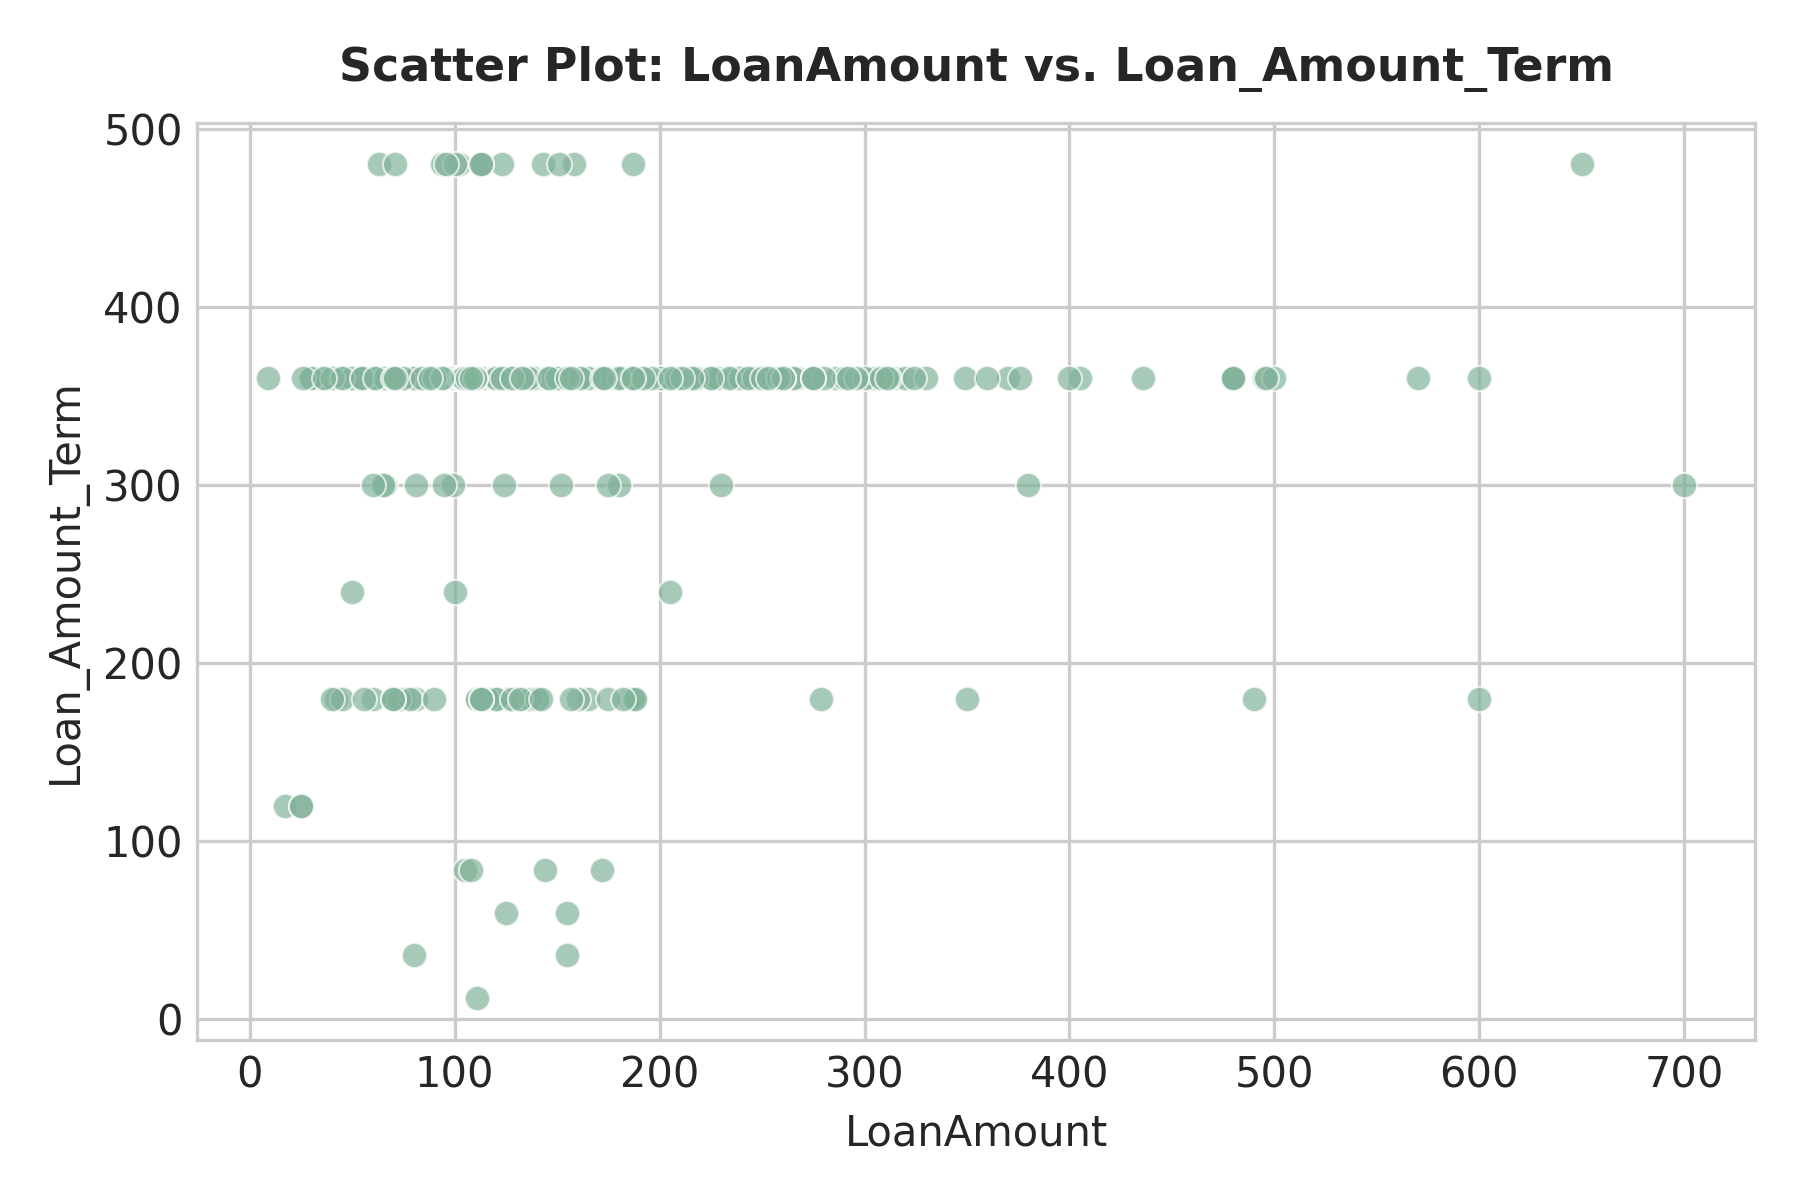
\includegraphics[width=0.75\linewidth]{figures_loan/scatter_LoanAmount_vs_Loan_Amount_Term.png}
\caption{Scatter Plot: Loan Amount vs. Loan Amount Term}
\label{fig:scatter_loan_term}
\end{figure}
\textbf{Inference:} Points align along discrete horizontal bands corresponding to standard term lengths (e.g. 180 and 360 months).

\begin{figure}[H]
\centering
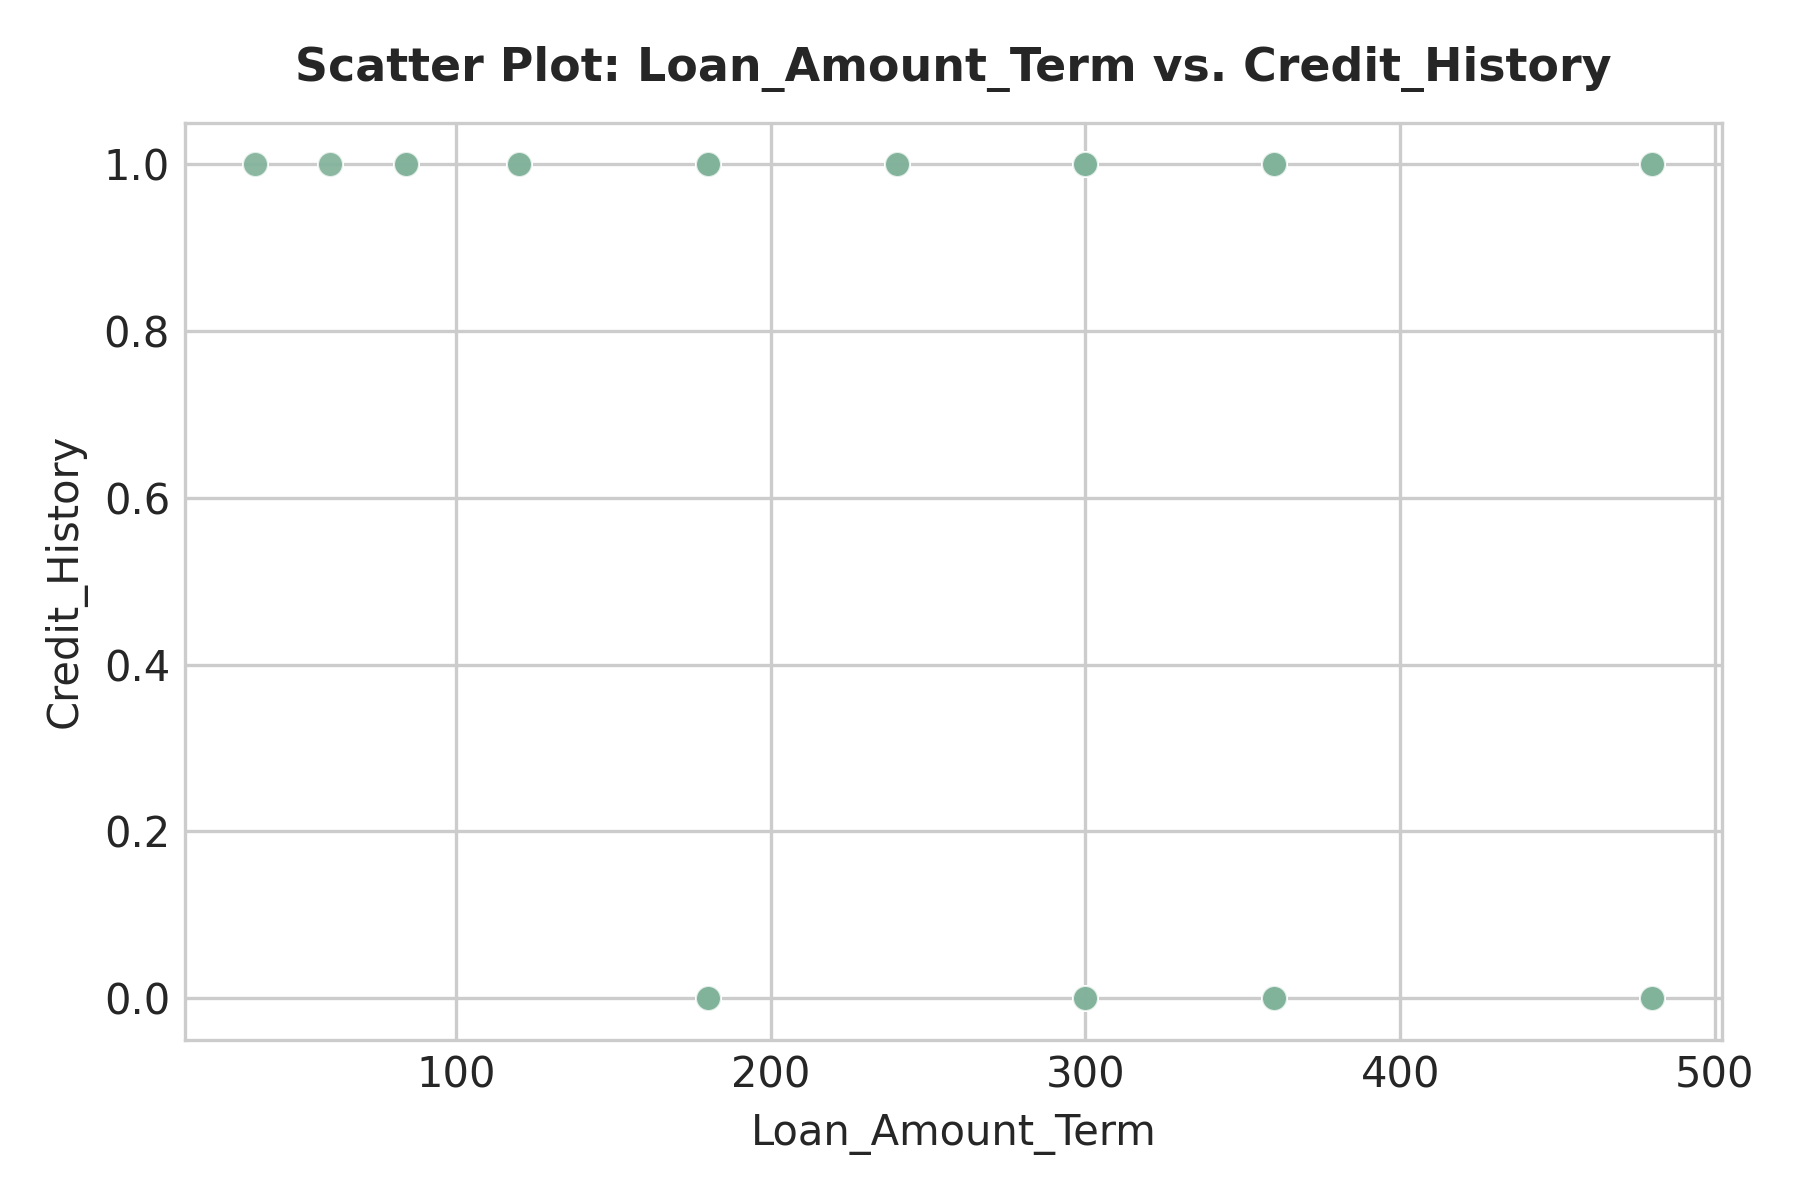
\includegraphics[width=0.75\linewidth]{figures_loan/scatter_Loan_Amount_Term_vs_Credit_History.png}
\caption{Scatter Plot: Loan Amount Term vs. Credit History}
\label{fig:scatter_term_history}
\end{figure}
\textbf{Inference:} Bivariate points are localized at discrete grid intersections, reflecting the categorical nature of both variables.

\section{Data Preprocessing}
The automated EDA framework handles essential preprocessing checks:
\begin{itemize}[noitemsep]
    \item \textbf{Type Profiling}: Automatically partitions columns into numerical, categorical, and text types.
    \item \textbf{Null Detection}: Identifies missing values across key columns (\texttt{Gender}, \texttt{Married}, \texttt{Dependents}, \texttt{Self\_Employed}, \texttt{LoanAmount}, \texttt{Loan\_Amount\_Term}, \texttt{Credit\_History}). Recommended resolution involves median imputation for numerical data and mode imputation for categorical attributes.
    \item \textbf{Duplicate Verification}: Checks for duplicate rows across samples (0 duplicates found).
    \item \textbf{Standardization}: Recommends z-score scaling ($z = \frac{x - \mu}{\sigma}$) prior to fitting distance-based models.
\end{itemize}

\section{Machine Learning Algorithms}
The table below categorizes the five benchmark datasets explored in this experiment according to task type, feature selection, and algorithm choices.

\begin{table}[H]
\centering
\caption{Benchmark Dataset Mapping and Model Selection}
\label{tab:dataset_mapping}
\begin{tabular}{p{3.5cm}p{3cm}p{3cm}p{4cm}}
\toprule
Dataset Name & Type of ML Task & Feature Selection & Suitable ML Algorithm \\
\midrule
Iris Dataset & Supervised Multiclass Classification & SelectKBest (ANOVA F-test) / PCA & Decision Trees, Support Vector Machines, KNN \\
Loan Amount Prediction & Supervised Regression & Correlation Analysis / Mutual Information & Linear Regression, Random Forest Regressor \\
Predicting Diabetes & Supervised Binary Classification & Chi-Square Test / SelectKBest & Logistic Regression, Support Vector Classifier \\
Classification of Email Spam & Supervised Binary Classification & Information Gain / TF-IDF Vectorization & Multinomial Naïve Bayes, SVM \\
Handwritten Character / MNIST & Supervised Multiclass Classification & Principal Component Analysis (PCA) & Convolutional Neural Networks (CNN), SVM \\
\bottomrule
\end{tabular}
\end{table}

\section{Experimental Setup}
All automated scripts and visualization modules were executed under the setup detailed below.

\begin{table}[H]
\centering
\begin{tabular}{ll}
\toprule
Component & Environment Specification \\
\midrule
Python Environment & Version 3.10+ \\
Pandas Library & Version 2.0+ \\
NumPy Library & Version 1.24+ \\
Matplotlib / Seaborn & Matplotlib 3.7+ / Seaborn 0.12+ \\
Execution Interface & Jupyter Notebook / Integrated Terminal \\
Operating System & Windows 11 \\
\bottomrule
\end{tabular}
\end{table}

\section{Hyperparameter Selection}
As this experiment focuses on automated exploratory analysis, hyperparameter tuning for predictive models was omitted. Visualization parameters were set as follows:
\begin{itemize}[noitemsep]
    \item \textbf{KDE Bandwidth}: Standard Gaussian kernel density estimator with automatic bandwidth calculation.
    \item \textbf{Histogram Binning}: Bins dynamically assigned based on the Freedman-Diaconis rule.
    \item \textbf{Correlation Matrix}: Pearson correlation coefficient ($r$) computed across numerical feature pairs.
\end{itemize}

\section{Results}
The automated pipeline extracted summary statistics across all numerical features in the Loan dataset.

\begin{table}[H]
\centering
\caption{Loan Dataset Descriptive Summary Statistics}
\label{tab:loan_stats}
\begin{tabular}{lcccc}
\toprule
Metric & ApplicantIncome & CoapplicantIncome & LoanAmount & Loan\_Amount\_Term \\
\midrule
Mean & \$5,403.46 & \$1,621.24 & \$146.41k & 342.00 months \\
Std Dev & \$6,109.04 & \$2,926.25 & \$85.59k & 65.12 months \\
Minimum & \$150.00 & \$0.00 & \$9.00k & 12.00 months \\
Median (50\%) & \$3,812.50 & \$1,188.50 & \$128.00k & 360.00 months \\
Maximum & \$81,000.00 & \$41,667.00 & \$700.00k & 480.00 months \\
\bottomrule
\end{tabular}
\end{table}

\section{Result Visualization}
All 28 visualization plots were exported cleanly to \texttt{figures\_loan/}. The analysis confirmed zero duplicate rows, identified skewness across financial features, and demonstrated a positive linear relationship ($r = 0.57$) between applicant income and requested credit amount.

\section{Discussion}
Automated exploratory tools provide fast, reproducible, and standardized data quality insights prior to model development.
\begin{itemize}[noitemsep]
    \item \textbf{Advantages}: Instantly surfaces missing values, feature skewness, and class imbalance without requiring manual plotting code.
    \item \textbf{Limitations}: Pairwise plotting scales quadratically ($\mathcal{O}(d^2)$) with feature count, which can increase memory overhead for high-dimensional data.
    \item \textbf{Future Extensions}: Incorporate interactive HTML dashboard generation (e.g. via Sweetviz or ydata-profiling) and automated outlier flags.
\end{itemize}

\section{Conclusion}
This experiment established an automated EDA workflow using core Python packages (NumPy, SciPy, Pandas, Matplotlib, Seaborn, and Scikit-Learn). Applied to the Loan dataset, the pipeline generated 28 diagnostic graphics revealing feature distributions, correlation patterns, and preprocessing needs. Additionally, five benchmark datasets were categorized into appropriate machine learning workflows, providing a solid foundation for model implementation.

\section{References}
\begin{enumerate}[label={[\arabic*]}, leftmargin=2em]
    \item Pandas Development Team, ``Pandas API Reference,'' \url{https://pandas.pydata.org/docs/reference/index.html}.
    \item NumPy Developers, ``NumPy User Guide,'' \url{https://numpy.org/doc/stable/user/index.html}.
    \item Seaborn Project, ``Seaborn: Statistical Data Visualization,'' \url{https://seaborn.pydata.org/}.
    \item UCI Machine Learning Repository, ``Loan Approval Dataset,'' \url{https://archive.ics.uci.edu/ml/index.php}.
\end{enumerate}

\end{document}
